% !TeX root = tcolorbox.tex
% include file of tcolorbox.tex (manual of the LaTeX package tcolorbox)
\clearpage
\section{Library \mylib{skins}}\label{sec:skins}
The library is loaded by a package option or inside the preamble by:
\begin{dispListing}
\tcbuselibrary{skins}
\end{dispListing}
This also loads the package |tikz| \cite{tantau:2013a}. Typically but not necessarily,
the following skins use |tikz| instead of |pgf|.

\subsection{Style Option Keys}\label{subsec:addstyleoptions}
The following style options are applicable for all skins which
use engines of type |path|, |pathfirst|, |pathmiddle|, or |pathlast|.
Especially, the skin \refSkin{enhanced} supports \emph{all} of them
and \refSkin{standard} \emph{none}.

\begin{docTcbKey}{frame style}{=\meta{\texttt{\upshape tikz} keys}}{style, no default}
  The \meta{\texttt{\upshape tikz} keys} are used inside the |tikz| path command
  for drawing the \emph{frame} of the box.\\
  This option is available if the \refKey{/tcb/frame engine} is set to
  |path|, |pathfirst|, |pathmiddle|, or |pathlast|.
  It is \emph{not} available for |standard|.
\begin{dispExample*}{sbs,lefthand ratio=0.66}
\tcbset{colback=red!5!white,fonttitle=\bfseries}

\begin{tcolorbox}[enhanced,title=My title,
  frame style={left color=red!75!black,
               right color=blue!75!black}]
This is a \textbf{tcolorbox}.
\tcblower
This is the lower part.
\end{tcolorbox}
\end{dispExample*}
\end{docTcbKey}


\begin{docTcbKey}{frame style image}{=\meta{file name}}{no default, initially unset}
  Fills the frame with an external image referenced by \meta{file name}.
  For advanced features like blending of a picture with the background,
  use \refKey{/tcb/frame style} together with \refKey{/tikz/fill stretch image}.
\begin{dispExample*}{sbs,lefthand ratio=0.66}
\tcbset{colback=red!5!white,fonttitle=\bfseries}

\begin{tcolorbox}[enhanced,title=My title,
  frame style image=blueshade.png]
This is a \textbf{tcolorbox}.
\tcblower
This is the lower part.
\end{tcolorbox}
\end{dispExample*}
\end{docTcbKey}

\clearpage
\begin{docTcbKey}{frame style tile}{=\marg{graphics options}\marg{file name}}{no default, initially unset}
  Fills the frame with a tile pattern based on an external image referenced by \meta{file name}.
  The \meta{graphics options} are given to the underlying \docAuxCommand*{includegraphics} command.
  For advanced features like blending of a picture with the background,
  use \refKey{/tcb/frame style} together with \refKey{/tikz/fill tile image}.
\begin{dispExample*}{sbs,lefthand ratio=0.66}
\tcbset{colback=red!5!white,coltitle=red!30!black,
  opacityback=0.75,fonttitle=\bfseries}

\begin{tcolorbox}[enhanced,title=My title,
  frame style tile={width=1cm}{pink_marble.png}]
This is a \textbf{tcolorbox}.
\tcblower
This is the lower part.
\end{tcolorbox}
\end{dispExample*}
\end{docTcbKey}


\begin{docTcbKey}{frame hidden}{}{style, no value}
  This is a shortcut for |frame style={draw=none,fill=none}|.
  Depending on the skin, this option switches off the drawing of the
  frame.
  Alternatively, use \refKey{/tcb/frame empty}.
\begin{dispExample*}{sbs,lefthand ratio=0.66}
\tcbset{colback=red!5!white,colframe=red!75!black,
  fonttitle=\bfseries,coltitle=black}

\begin{tcolorbox}[enhanced,title=My title,
  frame hidden]
This is a \textbf{tcolorbox}.
\tcblower
This is the lower part.
\end{tcolorbox}
\end{dispExample*}
\end{docTcbKey}


\begin{docTcbKey}{interior style}{=\meta{\texttt{\upshape tikz} keys}}{style, no default}
  The \meta{\texttt{\upshape tikz} keys} are used inside the |tikz| path command
  for drawing the \emph{interior} of the box. They are used for the titled
  and for the untitled version as well.\\
  This option is available if the \refKey{/tcb/interior titled engine}
  or \refKey{/tcb/interior engine} is set to
  |path|, |pathfirst|, |pathmiddle|, or |pathlast|.
  It is \emph{not} available for |standard|.
\begin{dispExample*}{sbs,lefthand ratio=0.66}
\tcbset{colframe=red!75!black,fonttitle=\bfseries}

\begin{tcolorbox}[enhanced,title=My title,
  interior style={left color=red!20!white,
                  right color=yellow!50!white}]
This is a \textbf{tcolorbox}.
\tcblower
This is the lower part.
\end{tcolorbox}
\end{dispExample*}
\end{docTcbKey}

\clearpage
\begin{docTcbKey}{interior style image}{=\meta{file name}}{no default, initially unset}
  Fills the interior with an external image referenced by \meta{file name}.
  For advanced features like blending of a picture with the background,
  use \refKey{/tcb/interior style} together with \refKey{/tikz/fill stretch image}.
\begin{dispExample*}{sbs,lefthand ratio=0.66}
\tcbset{colframe=red!75!black,fonttitle=\bfseries}

\begin{tcolorbox}[enhanced,title=My title,
  interior style image=goldshade.png]
This is a \textbf{tcolorbox}.
\tcblower
This is the lower part.
\end{tcolorbox}
\end{dispExample*}
\end{docTcbKey}


\begin{docTcbKey}{interior style tile}{=\marg{graphics options}\marg{file name}}{no default, initially unset}
  Fills the interior with a tile pattern based on an external image referenced by \meta{file name}.
  The \meta{graphics options} are given to the underlying \docAuxCommand*{includegraphics} command.
  For advanced features like blending of a picture with the background,
  use \refKey{/tcb/interior style} together with \refKey{/tikz/fill tile image}.

\begin{dispExample*}{sbs,lefthand ratio=0.66}
\tcbset{colframe=red!75!black,fonttitle=\bfseries}

\begin{tcolorbox}[enhanced,title=My title,
  interior style tile={width=2cm}{crinklepaper.png}]
This is a \textbf{tcolorbox}.
\tcblower
This is the lower part.
\end{tcolorbox}
\end{dispExample*}
\end{docTcbKey}


\begin{docTcbKey}{interior hidden}{}{style, no value}
  This is a shortcut for |interior style={draw=none,fill=none}|.
  Depending on the skin, this option switches off the drawing of the
  interior.
  Alternatively, use \refKey{/tcb/interior empty} and/or \refKey{/tcb/interior titled empty}.
\begin{dispExample*}{sbs,lefthand ratio=0.66}
\tcbset{frame style={top color=red!20!white,
  bottom color=red!20!white!75!black},
  fonttitle=\bfseries,coltitle=black}

\begin{tcolorbox}[enhanced,title=My title,
  interior hidden]
This is a \textbf{tcolorbox}.
\tcblower
This is the lower part.
\end{tcolorbox}
\end{dispExample*}
\end{docTcbKey}

\clearpage
\begin{docTcbKey}{segmentation style}{=\meta{\texttt{\upshape tikz} keys}}{style, no default}
  The \meta{\texttt{\upshape tikz} keys} are used inside the |tikz| path command
  for drawing the \emph{segmentation} line of the box.\\
  This option is available if the \refKey{/tcb/segmentation engine}
  is set to |path|.
  It is \emph{not} available for |standard|.
\begin{dispExample*}{sbs,lefthand ratio=0.66}
\tcbset{colback=red!5!white,colframe=red!75!black,
  fonttitle=\bfseries}

\begin{tcolorbox}[enhanced,title=My title,
  segmentation style={double=white,draw=blue,
                  double distance=1pt,solid}]
This is a \textbf{tcolorbox}.
\tcblower
This is the lower part.
\end{tcolorbox}
\end{dispExample*}
\end{docTcbKey}


\begin{docTcbKey}{segmentation hidden}{}{style, no value}
  This is a shortcut for |segmentation style={draw=none,fill=none}|.
  Depending on the skin, this option switches off the drawing of the
  segmentation line. See also \refKey{/tcb/lower separated} which
  has the same effect for most skins.
  Alternatively, use \refKey{/tcb/segmentation empty}.
\begin{dispExample*}{sbs,lefthand ratio=0.66}
\tcbset{colback=red!5!white,colframe=red!75!black,
  fonttitle=\bfseries}

\begin{tcolorbox}[title=My title,
  enhanced,segmentation hidden]
This is a \textbf{tcolorbox}.
\tcblower
This is the lower part.
\end{tcolorbox}
\end{dispExample*}
\end{docTcbKey}


\begin{docTcbKey}{title style}{=\meta{\texttt{\upshape tikz} keys}}{style, no default}
  The \meta{\texttt{\upshape tikz} keys} are used inside the |tikz| path command
  for drawing the \emph{title area} of the box.\\
  This option is available if the \refKey{/tcb/title engine} is set to
  |path|, |pathfirst|, |pathmiddle|, or |pathlast|.
  It is \emph{not} available for |standard|.
\begin{dispExample*}{sbs,lefthand ratio=0.66}
\tcbset{colback=red!5!white,colframe=red!75!black,
  coltitle=blue!50!black,fonttitle=\bfseries}

\begin{tcolorbox}[enhanced,title=My title,
  title style={left color=blue!15!yellow,
               right color=red!85!black}]
This is a \textbf{tcolorbox}.
\tcblower
This is the lower part.
\end{tcolorbox}
\end{dispExample*}
\end{docTcbKey}

\clearpage
\begin{docTcbKey}{title style image}{=\meta{file name}}{no default, initially unset}
  Fills the title area with an external image referenced by \meta{file name}.
  For advanced features like blending of a picture with the background,
  use \refKey{/tcb/title style} together with \refKey{/tikz/fill stretch image}.

\begin{dispExample*}{sbs,lefthand ratio=0.66}
\tcbset{colback=blue!5!white,colframe=blue!75!black,
  fonttitle=\bfseries}

\begin{tcolorbox}[enhanced,title=My title,
  title style image=blueshade.png]
This is a \textbf{tcolorbox}.
\tcblower
This is the lower part.
\end{tcolorbox}
\end{dispExample*}
\end{docTcbKey}


\begin{docTcbKey}{title style tile}{=\marg{graphics options}\marg{file name}}{no default, initially unset}
  Fills the title area with a tile pattern based on an external image referenced by \meta{file name}.
  The \meta{graphics options} are given to the underlying \docAuxCommand*{includegraphics} command.
  For advanced features like blending of a picture with the background,
  use \refKey{/tcb/title style} together with \refKey{/tikz/fill tile image}.

\begin{dispExample*}{sbs,lefthand ratio=0.66}
\tcbset{colback=red!5!white,colframe=red!75!black,
  coltitle=blue!50!black,fonttitle=\bfseries}

\begin{tcolorbox}[enhanced,title=My title,
  title style tile={width=1cm}{pink_marble.png}]
This is a \textbf{tcolorbox}.
\tcblower
This is the lower part.
\end{tcolorbox}
\end{dispExample*}
\end{docTcbKey}


\begin{docTcbKey}{title hidden}{}{style, no value}
  This is a shortcut for |title style={draw=none,fill=none}|.
  Depending on the skin, this option switches off the drawing of the
  title background. See also \refKey{/tcb/title filled} for a similar effect.
  Alternatively, use \refKey{/tcb/title empty}.
\begin{dispExample*}{sbs,lefthand ratio=0.66}
\tcbset{colback=red!5!white,colframe=red!75!black,
  fonttitle=\bfseries}

\begin{tcolorbox}[title=My title,
  enhanced,title hidden]
This is a \textbf{tcolorbox}.
\tcblower
This is the lower part.
\end{tcolorbox}
\end{dispExample*}
\end{docTcbKey}

\clearpage

The combined \tikzname\ style applied to frame, interior, and title
background can used by authors in customizing code.

\begin{docTikzKey}{tcb fill frame}{}{style, no value}
This is a \tikzname\ style which is finally applied to the \emph{frame}
of the box.

\begin{dispExample*}{sbs,lefthand ratio=0.66}
% \tcbuselibrary{hooks}
\tcbset{enhanced,colback=red!5!white,
  colframe=red!75!black,fonttitle=\bfseries,
  frame code app={\path[tcb fill frame]
    ([yshift=-2mm]frame.north)
        circle (8mm); }  }

\begin{tcolorbox}[title=My title]
This is a \textbf{tcolorbox}.
\tcblower
This is the lower part.
\end{tcolorbox}
\end{dispExample*}
\end{docTikzKey}


\begin{docTikzKey}{tcb fill interior}{}{style, no value}
This is a \tikzname\ style which is finally applied to the \emph{interior}
of the box.

\begin{dispExample*}{sbs,lefthand ratio=0.66}
% \tcbuselibrary{hooks}
\tcbset{enhanced,colback=red!5!white,
  colframe=red!75!black,fonttitle=\bfseries,
  interior titled code app={\path[tcb fill interior]
      ([yshift=-0.1pt]interior.north east)
    --([yshift=3pt]interior.north)
    --([yshift=-0.1pt]interior.north west)
    --cycle;}  }

\begin{tcolorbox}[title=My title]
This is a \textbf{tcolorbox}.
\tcblower
This is the lower part.
\end{tcolorbox}
\end{dispExample*}
\end{docTikzKey}


\begin{docTikzKey}{tcb fill title}{}{style, no value}
This is a \tikzname\ style which is finally applied to the \emph{title area}
of the box.

\begin{dispExample*}{sbs,lefthand ratio=0.66}
% \tcbuselibrary{hooks}
\tcbset{enhanced,colback=red!5!white,
  colframe=red!75!black,fonttitle=\bfseries,
  colbacktitle=blue!75!black,
  title code app={\path[tcb fill title]
    (title) circle (5mm); }  }

\begin{tcolorbox}[title=My title]
This is a \textbf{tcolorbox}.
\tcblower
This is the lower part.
\end{tcolorbox}
\end{dispExample*}
\end{docTikzKey}


\clearpage
\subsection{Boxed Title Option Keys}\label{subsec:skinboxedtitle}

The following options place the title text into an own \refCom{tcbox}.
This boxed title can be customized independently from the main box using
\refKey{/tcb/boxed title style}.
The placement can be influenced by \meta{boxtitle options}.

\begin{docTcbKey}{attach boxed title to top left}{\colOpt{=\meta{boxtitle options}}}{style, default empty}
The title is boxed with a \refCom{tcbox} and attached to
the top left corner of the main box.
\begin{dispExample*}{sbs,lefthand ratio=0.66}
\begin{tcolorbox}[enhanced,title=My title,
  attach boxed title to top left]
  This is a \textbf{tcolorbox}.
\end{tcolorbox}
\end{dispExample*}
\end{docTcbKey}

\begin{docTcbKey}{attach boxed title to top center}{\colOpt{=\meta{boxtitle options}}}{style, default empty}
The title is boxed with a \refCom{tcbox} and attached to
the top of the main box.
\begin{dispExample*}{sbs,lefthand ratio=0.66}
\begin{tcolorbox}[enhanced,title=My title,
  attach boxed title to top center]
  This is a \textbf{tcolorbox}.
\end{tcolorbox}
\end{dispExample*}
\end{docTcbKey}

\begin{docTcbKey}{attach boxed title to top right}{\colOpt{=\meta{boxtitle options}}}{style, default empty}
The title is boxed with a \refCom{tcbox} and attached to
the top right corner of the main box.
\begin{dispExample*}{sbs,lefthand ratio=0.66}
\begin{tcolorbox}[enhanced,title=My title,
  attach boxed title to top right]
  This is a \textbf{tcolorbox}.
\end{tcolorbox}
\end{dispExample*}
\end{docTcbKey}

\begin{docTcbKey}{attach boxed title to bottom left}{\colOpt{=\meta{boxtitle options}}}{style, default empty}
The title is boxed with a \refCom{tcbox} and attached to
the bottom left corner of the main box.
\begin{dispExample*}{sbs,lefthand ratio=0.66}
\begin{tcolorbox}[enhanced,title=My title,
  attach boxed title to bottom left]
  This is a \textbf{tcolorbox}.
\end{tcolorbox}
\end{dispExample*}
\end{docTcbKey}

\begin{docTcbKey}{attach boxed title to bottom center}{\colOpt{=\meta{boxtitle options}}}{style, default empty}
The title is boxed with a \refCom{tcbox} and attached to
the bottom of the main box.
\begin{dispExample*}{sbs,lefthand ratio=0.66}
\begin{tcolorbox}[enhanced,title=My title,
  attach boxed title to bottom center]
  This is a \textbf{tcolorbox}.
\end{tcolorbox}
\end{dispExample*}
\end{docTcbKey}

\begin{docTcbKey}{attach boxed title to bottom right}{\colOpt{=\meta{boxtitle options}}}{style, default empty}
The title is boxed with a \refCom{tcbox} and attached to
the bottom right corner of the main box.
\begin{dispExample*}{sbs,lefthand ratio=0.66}
\begin{tcolorbox}[enhanced,title=My title,
  attach boxed title to bottom right]
  This is a \textbf{tcolorbox}.
\end{tcolorbox}
\end{dispExample*}
\end{docTcbKey}

\clearpage

The \meta{boxtitle options} of the keys described above are shift values.
The dimensions of the boxed title are stored into two macros
\docAuxCommand{tcboxedtitleheight} and
\docAuxCommand{tcboxedtitlewidth}. These macros can be used inside the
following \meta{boxtitle options}:

\begin{boxTcbKey}{xshift}{=\meta{length}}{no default, initially |0pt|}
The boxed title is shifted by \meta{length} in the horizontal direction.
\begin{dispExample*}{sbs,lefthand ratio=0.66}
\begin{tcolorbox}[enhanced,title=My title,
  attach boxed title to top left={xshift=-2mm},
  boxed title style={size=small,colback=blue}]
  This is a \textbf{tcolorbox}.
\end{tcolorbox}
\end{dispExample*}
\end{boxTcbKey}

\begin{boxTcbKey}{yshift}{=\meta{length}}{no default, initially |0pt|}
The boxed title is shifted by \meta{length} in the vertical direction.
\begin{dispExample*}{sbs,lefthand ratio=0.66}
\begin{tcolorbox}[enhanced,title=My title,
  attach boxed title to top center=
    {yshift=-\tcboxedtitleheight/2},
  boxed title style={size=small,colback=blue}]
  This is a \textbf{tcolorbox}.
\end{tcolorbox}
\end{dispExample*}
\end{boxTcbKey}

\begin{boxTcbKey}{yshifttext}{=\meta{length}}{no default, initially |0pt|}
The text inside the main box by \meta{length} to give room for e.\,g.\ a sunken title.
\begin{dispExample*}{sbs,lefthand ratio=0.66}
\begin{tcolorbox}[enhanced,title=My title,
  attach boxed title to top center=
    {yshift=-3mm,yshifttext=-1mm},
  boxed title style={size=small,colback=blue}]
  This is a \textbf{tcolorbox}.
\end{tcolorbox}
\end{dispExample*}
\end{boxTcbKey}

\begin{boxTcbKey}{yshift*}{=\meta{length}}{no default, initially |0pt|}
Sets \refKey{/tcb/boxtitle/yshift} and \refKey{/tcb/boxtitle/yshifttext}
the same time.\\
\refKey{/tcb/boxtitle/yshifttext} is only set if necessary.
\begin{dispExample*}{sbs,lefthand ratio=0.66}
\begin{tcolorbox}[enhanced,title=My title,
  attach boxed title to top center={yshift*=-3mm},
  boxed title style={size=small,colback=blue}]
  This is a \textbf{tcolorbox}.
\end{tcolorbox}
\end{dispExample*}
\end{boxTcbKey}

\begin{marker}
The bounding box of the resulting total |tcolorbox| is adapted automatically to the
\emph{vertical} dimensions of the boxed title. Possible horizontal enlargements
are \emph{not} automatically computed.
\end{marker}


\begin{dispExample*}{sbs,lefthand ratio=0.66}
\begin{tcolorbox}[enhanced,title=My title,
  attach boxed title to top left=
    {xshift=-2mm,yshift=-2mm},
  boxed title style={size=small,colback=blue},
  show bounding box]
  This is a \textbf{tcolorbox}.
\end{tcolorbox}
\end{dispExample*}


\clearpage
\begin{marker}
  The boxed title options are implemented as an underlay, see \Vref{subsec:skinunderlay}.
  Therefore, a boxed title is not drawn, if a skin does not support underlays
  like \refSkin{standard}. Still, the room for the boxed
  titles gets reserved in these cases.
\end{marker}

\begin{marker}
  A \tikzname\ node |title| is produced by a boxed title which can be used
  inside \refKey{/tcb/frame code}, \refKey{/tcb/interior code},
  underlays, overlays, and finishes.
\end{marker}

\begin{marker}
  A boxed title is almost always the first underlay. The only exceptions are
  underlays defined by \refKey{/tcb/underlay boxed title} which are drawn
  before. Additionally, underlays defined by \refKey{/tcb/underlay boxed title}
  are only drawn, if a boxed title is actually set. They are ignored, if
  there is no boxed title.
\end{marker}



\begin{docTcbKey}{boxed title style}{=\meta{options}}{style, initially empty}
By default, a boxed title is dimensioned with \refKey{/tcb/size}|=|\docValue*{title}
and inherits \refKey{/tcb/colframe} of the main box.
Also, the \refKey{/tcb/colback} is inherited from the main \refKey{/tcb/colbacktitle}.
Font and color of the title text are set as usual.
All other \meta{options} are set by the |boxed title style| key.
Since a boxed title is set by \refCom{tcbox}, all |tcolorbox| options are
applicable here.

\begin{dispExample*}{sbs,lefthand ratio=0.66}
\begin{tcolorbox}[enhanced,title=My title,
  fonttitle=\bfseries,coltitle=green!25!black,
  attach boxed title to top center=
    {yshift=-2mm,yshifttext=-1mm},
  boxed title style={colframe=green!75!black,
    colback=yellow!50!green}]
  This is a \textbf{tcolorbox}.
\end{tcolorbox}
\end{dispExample*}


\begin{dispExample*}{sbs,lefthand ratio=0.66}
\begin{tcolorbox}[enhanced,title=My title,
  colframe=red!50!black,colback=red!10!white,
  arc=1mm,colbacktitle=red!10!white,
  fonttitle=\bfseries,coltitle=red!50!black,
  attach boxed title to top left=
    {xshift=3.2mm,yshift=-0.50mm},
  boxed title style={enhanced,
    skin=enhancedfirst jigsaw,
    size=small,arc=1mm,bottom=-1mm,
    interior style={top color=red!30!white,
      bottom color=red!20!white}}]
  This is a \textbf{tcolorbox}.
\end{tcolorbox}
\end{dispExample*}

\begin{dispExample}
\begin{tcolorbox}[enhanced,title=My title,
  colframe=blue!50!black,colback=blue!10!white,colbacktitle=blue!5!yellow!10!white,
  fonttitle=\bfseries,coltitle=black,attach boxed title to top center=
    {yshift=-0.25mm-\tcboxedtitleheight/2,yshifttext=2mm-\tcboxedtitleheight/2},
  boxed title style={enhanced,boxrule=0.5mm,
    frame code={ \path[tcb fill frame] ([xshift=-4mm]frame.west)
    -- (frame.north west) -- (frame.north east) -- ([xshift=4mm]frame.east)
    -- (frame.south east) -- (frame.south west) -- cycle; },
    interior code={ \path[tcb fill interior] ([xshift=-2mm]interior.west)
    -- (interior.north west) -- (interior.north east)
    -- ([xshift=2mm]interior.east) -- (interior.south east) -- (interior.south west)
    -- cycle;}  }]
  \lipsum[2]
\end{tcolorbox}
\end{dispExample}


\begin{dispExample}
% \usepackage{varwidth}
\newtcolorbox{mybox}[2][]{enhanced,skin=enhancedlast jigsaw,
  attach boxed title to top left={xshift=-4mm,yshift=-0.5mm},
  fonttitle=\bfseries\sffamily,varwidth boxed title=0.7\linewidth,
  colbacktitle=blue!45!white,colframe=red!50!black,
  interior style={top color=blue!10!white,bottom color=red!10!white},
  boxed title style={empty,arc=0pt,outer arc=0pt,boxrule=0pt},
  underlay boxed title={
    \fill[blue!45!white] (title.north west) -- (title.north east)
      -- +(\tcboxedtitleheight-1mm,-\tcboxedtitleheight+1mm)
      -- ([xshift=4mm,yshift=0.5mm]frame.north east) -- +(0mm,-1mm)
      -- (title.south west) -- cycle;
    \fill[blue!45!white!50!black] ([yshift=-0.5mm]frame.north west)
      -- +(-0.4,0) -- +(0,-0.3) -- cycle;
    \fill[blue!45!white!50!black] ([yshift=-0.5mm]frame.north east)
      -- +(0,-0.3) -- +(0.4,0) -- cycle;  },
  title={#2},#1}

\begin{mybox}{My title}
  \lipsum[2]
\end{mybox}
\end{dispExample}


\begin{dispExample}
% \usepackage{varwidth}
\newtcolorbox{mybox}[2][]{enhanced,
  attach boxed title to top left={xshift=1cm,yshift=-2mm},
  fonttitle=\bfseries,varwidth boxed title=0.7\linewidth,
  colbacktitle=green!45!white,coltitle=green!10!black,colframe=green!50!black,
  interior style={top color=yellow!10!white,bottom color=green!10!white},
  boxed title style={enhanced,boxrule=0.75mm,colframe=white,
    borderline={0.1mm}{0mm}{green!50!black},
    borderline={0.1mm}{0.75mm}{green!50!black},
    interior style={top color=green!10!white,bottom color=green!10!white,
      middle color=green!50!white},
    drop fuzzy shadow},
  title={#2},#1}

\begin{mybox}{My title}
  \lipsum[2]
\end{mybox}
\end{dispExample}


\begin{dispExample}
% \usepackage{varwidth}
\newtcolorbox{mybox}[2][]{skin=enhancedlast jigsaw,interior hidden,
  boxsep=0pt,top=0pt,colframe=red,coltitle=red!50!black,
  fonttitle=\bfseries\sffamily,
  attach boxed title to bottom center,
  boxed title style={empty,boxrule=0.5mm},
  varwidth boxed title=0.5\linewidth,
  underlay boxed title={
    \draw[white,line width=0.5mm]
      ([xshift=0.3mm-\tcboxedtitleheight*2,yshift=0.3mm]title.north west)
      --([xshift=-0.3mm+\tcboxedtitleheight*2,yshift=0.3mm]title.north east);
    \path[draw=red,top color=white,bottom color=red!50!white,line width=0.5mm]
    ([xshift=0.25mm-\tcboxedtitleheight*2,yshift=0.25mm]title.north west)
    cos +(\tcboxedtitleheight,-\tcboxedtitleheight/2)
    sin +(\tcboxedtitleheight,-\tcboxedtitleheight/2)
    -- ([xshift=0.25mm,yshift=0.25mm]title.south west)
    -- ([yshift=0.25mm]title.south east)
    cos +(\tcboxedtitleheight,\tcboxedtitleheight/2)
    sin +(\tcboxedtitleheight,\tcboxedtitleheight/2); },
  title={#2},#1}

\begin{mybox}{My title}
  \lipsum[2]
\end{mybox}
\end{dispExample}
\end{docTcbKey}


\clearpage
\begin{docTcbKey}{hbox boxed title}{}{no value, initially set}
The title text content is captured with a horizontal box.
Especially, there are no linebreak possible.
\begin{dispExample*}{sbs,lefthand ratio=0.66}
\newtcolorbox{mybox}[1]{hbox boxed title,
  enhanced,attach boxed title to top center=
    {yshift=-3mm,yshifttext=-1mm},
  boxed title style={size=small,colback=red},
  title={#1}}

\begin{mybox}{Short title}
  This is a \textbf{tcolorbox}.
\end{mybox}\bigskip

\begin{mybox}{This title is not really very short}
  This is a \textbf{tcolorbox}.
\end{mybox}
\end{dispExample*}
\end{docTcbKey}


\begin{docTcbKey}{minipage boxed title}{\colOpt{=\meta{length}}}{initially unset}
The title text content is captured with a minipage with a width of \meta{length}.
By default, the resulting boxed title is somewhat smaller than the main box.
\begin{dispExample*}{sbs,lefthand ratio=0.66}
\newtcolorbox{mybox}[1]{minipage boxed title,
  enhanced,attach boxed title to top center=
    {yshift=-3mm,yshifttext=-1mm},
  boxed title style={size=small,colback=red},
  center title,title={#1}}

\begin{mybox}{Short title}
  This is a \textbf{tcolorbox}.
\end{mybox}\bigskip

\begin{mybox}{This title is not really very short}
  This is a \textbf{tcolorbox}.
\end{mybox}
\end{dispExample*}
\end{docTcbKey}


\begin{docTcbKey}{minipage boxed title*}{\colOpt{=\meta{length}}}{initially unset}
The title text content is captured with a minipage with a width of main box width plus \meta{length}.
By default, the resulting boxed title is somewhat smaller than the main box.
\begin{dispExample*}{sbs,lefthand ratio=0.66}
\newtcolorbox{mybox}[1]{minipage boxed title*=-2cm,
  enhanced,attach boxed title to top center=
    {yshift=-3mm,yshifttext=-1mm},
  boxed title style={size=small,colback=red},
  center title,title={#1}}

\begin{mybox}{Short title}
  This is a \textbf{tcolorbox}.
\end{mybox}\bigskip

\begin{mybox}{This title is not really very short}
  This is a \textbf{tcolorbox}.
\end{mybox}
\end{dispExample*}
\end{docTcbKey}


\clearpage
\begin{docTcbKey}{tikznode boxed title}{=\meta{options}}{initially unset}
The title text content is captured with a \tikzname\ node with given \tikzname\ \meta{options}.
The text is centered by default
\begin{dispExample*}{sbs,lefthand ratio=0.66}
\newtcolorbox{mybox}[1]{tikznode boxed title,
  enhanced,attach boxed title to top center=
    {yshift=-3mm,yshifttext=-1mm},
  boxed title style={size=small,colback=red},
  title={#1}}

\begin{mybox}{Short title}
  This is a \textbf{tcolorbox}.
\end{mybox}\bigskip

\begin{mybox}{This title\\is not really\\very short}
  This is a \textbf{tcolorbox}.
\end{mybox}
\end{dispExample*}
\end{docTcbKey}


\begin{docTcbKey}{varwidth boxed title}{\colOpt{=\meta{length}}}{initially unset}
The title text content is captured with a |varwidth| environment with a width of \meta{length}.
This style needs the |varwidth| package \cite{arseneau:2011a} to be loaded manually.
By default, the resulting boxed title is somewhat smaller than the main box.
\begin{dispExample*}{sbs,lefthand ratio=0.66}
% \usepackage{varwidth}
\newtcolorbox{mybox}[1]{varwidth boxed title,
  enhanced,attach boxed title to top center=
    {yshift=-3mm,yshifttext=-1mm},
  boxed title style={size=small,colback=red},
  center title,title={#1}}

\begin{mybox}{Short title}
  This is a \textbf{tcolorbox}.
\end{mybox}\bigskip

\begin{mybox}{This title is not really very short}
  This is a \textbf{tcolorbox}.
\end{mybox}
\end{dispExample*}
\end{docTcbKey}


\begin{docTcbKey}{varwidth boxed title*}{\colOpt{=\meta{length}}}{initially unset}
The title text content is captured with a |varwidth| environment with a width of main box width plus \meta{length}.
This style needs the |varwidth| package \cite{arseneau:2011a} to be loaded manually.
By default, the resulting boxed title is somewhat smaller than the main box.
\begin{dispExample*}{sbs,lefthand ratio=0.66}
% \usepackage{varwidth}
\newtcolorbox{mybox}[1]{varwidth boxed title*=-2cm,
  enhanced,attach boxed title to top center=
    {yshift=-3mm,yshifttext=-1mm},
  boxed title style={size=small,colback=red},
  center title,title={#1}}

\begin{mybox}{Short title}
  This is a \textbf{tcolorbox}.
\end{mybox}\bigskip

\begin{mybox}{This title is not really very short}
  This is a \textbf{tcolorbox}.
\end{mybox}
\end{dispExample*}
\end{docTcbKey}


\clearpage
\subsection{Watermark Option Keys}\label{subsec:watermarks}
The following watermark options are applicable for all skins which
use |tikzpicture| as \refKey{/tcb/graphical environment}.
Therefore, the skin \refSkin{standard} does not support these watermarks,
but all other skins, e.\,g.\ \refSkin{enhanced}.

\begin{marker}
The watermark options rely on the more general overlay options described in
Section \ref{subsec:overlays} from page \pageref{subsec:overlays}.
Therefore, \emph{watermarks} and \emph{overlays} cannot be used mixed.
But a mixture is possible with the \mylib{hooks} library, see Section \ref{sec:hooks}.
\end{marker}


\begin{docTcbKey}{watermark text}{=\meta{text}}{no default, initially unset}
  Writes some \meta{text} in the center of the interior region of a |tcolorbox|.
  This \meta{text} is written \emph{after} the
  frame and interior are drawn and \emph{before} the text content is drawn.
  It is zoomed or stretched according the values of
  \refKey{/tcb/watermark zoom} or \refKey{/tcb/watermark stretch}.
\begin{dispExample}
\tcbset{colback=red!5!white,colframe=red!75!black,fonttitle=\bfseries}

\begin{tcolorbox}[enhanced,title=My title,watermark text=My Watermark]
\lipsum[1]
\tcblower
\lipsum[2]
\end{tcolorbox}
\end{dispExample}
\end{docTcbKey}

\enlargethispage*{1cm}

\begin{docTcbKey}{watermark text on}{=\meta{part} is \meta{text}}{no default, initially unset}
  This option writes some \meta{text} in the center of the interior region of a |tcolorbox|
  as described for \refKey{/tcb/watermark text}.
  But this is done only for boxes named \meta{part} of a break sequence, see
  \refKey{/tcb/breakable}.\\ 
  Feasible values for \meta{part} are:
  \begin{itemize}
  \item\docValue{broken}: all broken box parts,
  \item\docValue{unbroken}: unbroken boxes only,
  \item\docValue{first}: first parts of a break sequence,
  \item\docValue{middle}: middle parts of a break sequence,
  \item\docValue{last}: last parts of a break sequence,
  \item\docValue{unbroken and first}: unbroken boxes and first parts of a break sequence,
  \item\docValue{middle and last}: middle and last parts of a break sequence.
  \item\docValue{first and middle}: first and middle parts of a break sequence.
  \end{itemize}
\end{docTcbKey}


\clearpage


\begin{docTcbKey}{watermark graphics}{=\meta{file name}}{no default, initially unset}
  Draws an external picture referenced by \meta{file name}
  in the center of the interior region of a |tcolorbox|.
  The picture is drawn \emph{after} the
  frame and interior are drawn and \emph{before} the text content is drawn.
  It is zoomed or stretched according the values of
  \refKey{/tcb/watermark zoom} or \refKey{/tcb/watermark stretch}.
\begin{dispExample}
\tcbset{colback=red!5!white,colframe=red!75!black,fonttitle=\bfseries}

\begin{tcolorbox}[enhanced,title=My title,watermark graphics=Basilica_5.png,
  watermark opacity=0.15]
\lipsum[1-2]
\tcblower
This example uses a public domain picture from\\
\url{http://commons.wikimedia.org/wiki/File:Basilica_5.png}
\end{tcolorbox}
\end{dispExample}
\end{docTcbKey}


\begin{docTcbKey}{watermark graphics on}{=\meta{part} is \meta{file name}}{no default, initially unset}
  This option draws a picture referenced by \meta{file name} in the center of the interior region of a |tcolorbox|
  as described for \refKey{/tcb/watermark graphics}.
  But this is done only for boxes named \meta{part} of a break sequence, see
  \refKey{/tcb/breakable}.\\ 
  Feasible values for \meta{part} are:
  \begin{itemize}
  \item\docValue{broken}: all broken box parts,
  \item\docValue{unbroken}: unbroken boxes only,
  \item\docValue{first}: first parts of a break sequence,
  \item\docValue{middle}: middle parts of a break sequence,
  \item\docValue{last}: last parts of a break sequence,
  \item\docValue{unbroken and first}: unbroken boxes and first parts of a break sequence,
  \item\docValue{middle and last}: middle and last parts of a break sequence.
  \end{itemize}
\end{docTcbKey}



\clearpage
\begin{docTcbKey}{watermark tikz}{=\meta{graphical code}}{no default, initially unset}
  Draws the given |tikz| \meta{graphical code}
  in the center of the interior region of a |tcolorbox|.
  The code is executed \emph{after} the
  frame and interior are drawn and \emph{before} the text content is drawn.
  The result is zoomed or stretched according the values of
  \refKey{/tcb/watermark zoom} or \refKey{/tcb/watermark stretch}.
\begin{dispExample}
\tcbset{colback=red!5!white,colframe=red!75!black,fonttitle=\bfseries}

\begin{tcolorbox}[enhanced,title=My title,
  watermark tikz={\draw[line width=2mm] circle (1cm)
    node{\fontfamily{ptm}\fontseries{b}\fontsize{20mm}{20mm}\selectfont ?};}]
\lipsum[1]
\tcblower
\lipsum[2]
\end{tcolorbox}
\end{dispExample}
\end{docTcbKey}



\begin{docTcbKey}{watermark tikz on}{=\meta{part} is \meta{graphical code}}{no default, initially unset}
  This option draws the given |tikz| \meta{graphical code} in the center of the interior region of a |tcolorbox|
  as described for \refKey{/tcb/watermark tikz}.
  But this is done only for boxes named \meta{part} of a break sequence, see
  \refKey{/tcb/breakable}.\\ 
  Feasible values for \meta{part} are:
  \begin{itemize}
  \item\docValue{broken}: all broken box parts,
  \item\docValue{unbroken}: unbroken boxes only,
  \item\docValue{first}: first parts of a break sequence,
  \item\docValue{middle}: middle parts of a break sequence,
  \item\docValue{last}: last parts of a break sequence,
  \item\docValue{unbroken and first}: unbroken boxes and first parts of a break sequence,
  \item\docValue{middle and last}: middle and last parts of a break sequence.
  \end{itemize}
\end{docTcbKey}


\begin{docTcbKey}{no watermark}{}{style, no default, initially set}
  Removes the watermark if set before. This is an alias for
  \refKey{/tcb/no overlay}.
\end{docTcbKey}


\clearpage
\begin{docTcbKey}{watermark opacity}{=\meta{fraction}}{no default, initially |1.00|}
  Sets the opacity value $\in[0,1]$ for a watermark.
\begin{dispExample}
\tcbset{enhanced,colback=red!5!white,colframe=red!75!black,fonttitle=\bfseries,
  watermark text=Watermark,nobeforeafter,width=(\linewidth-2mm)/2}

\begin{tcolorbox}[title=Opacity 1.00,watermark opacity=1.00]
\lipsum[2]
\end{tcolorbox}\hfill%
\begin{tcolorbox}[title=Opacity 0.50,watermark opacity=0.50]
\lipsum[2]
\end{tcolorbox}%
\end{dispExample}
\end{docTcbKey}

\enlargethispage{5mm}
\begin{docTcbKey}{watermark zoom}{=\meta{fraction}}{no default, initially |0.75|}
  Sets the zoom value for a watermark. The zoom respects the aspect ratio.
  The value $1.0$ means to fill the whole box until the watermark touches the frame.
\begin{dispExample}
\tcbset{enhanced,colback=red!5!white,colframe=red!75!black,fonttitle=\bfseries,
  watermark text=Watermark,nobeforeafter,width=(\linewidth-2mm)/2}

\begin{tcolorbox}[title=Zoom 1.0,watermark zoom=1.0]
\lipsum[2]
\end{tcolorbox}\hfill%
\begin{tcolorbox}[title=Zoom 0.5,watermark zoom=0.5]
\lipsum[2]
\end{tcolorbox}%
\end{dispExample}
\end{docTcbKey}

\clearpage

\begin{docTcbKey}{watermark shrink}{=\meta{fraction}}{no default, initially unset}
  Identically to \refKey{/tcb/watermark zoom}, but the watermark
  never gets enlarged. Thus, the watermark keeps its original size or is shrunk.
\end{docTcbKey}


\begin{docTcbKey}{watermark overzoom}{=\meta{fraction}}{no default, initially unset}
  Sets the overzoom value for a watermark. The overzoom respects the aspect ratio.
  The value $1.0$ means to fill the whole box until the watermark touches
  all four sides of the frame.
\begin{dispExample}
\tcbset{enhanced,colback=white,colframe=blue!50!black,fonttitle=\bfseries,
  watermark opacity=0.5,
  watermark graphics=lichtspiel.jpg,nobeforeafter,width=(\linewidth-2mm)/2}

\begin{tcolorbox}[title=Zoom 1.0,watermark zoom=1.0]
\lipsum[1]
\end{tcolorbox}\hfill%
\begin{tcolorbox}[title=Overzoom 1.0,watermark overzoom=1.0]
\lipsum[1]
\end{tcolorbox}%
\end{dispExample}
\end{docTcbKey}

\begin{marker}
If a \refKey{/tcb/watermark overzoom} value of |1.0| is used in connection
with invisible top and bottom rules which still have a thickness greater than |0pt|,
the space of these invisible rules may not be covered by the watermark.
For example, this situation may occur during the breaking of \refKey{/tcb/enhanced} boxes.
To avoid this optical glitch, just set \refKey{/tcb/pad at break} to any desired value.
\end{marker}

\clearpage
\begin{docTcbKey}{watermark stretch}{=\meta{fraction}}{no default, initially unset}
  Sets the stretch value for a watermark. The stretch value is applied to width
  and height in relation to the box dimensions. It does not respect the aspect ratio.
  The value $1.0$ means to fill the whole box.
\begin{dispExample}
\tcbset{enhanced,colback=white,colframe=blue!50!black,fonttitle=\bfseries,
  watermark graphics=lichtspiel.jpg,watermark opacity=0.5,
  nobeforeafter,width=(\linewidth-2mm)/2}

\begin{tcolorbox}[title=Stretch 1.00,watermark stretch=1.00]
\lipsum[2]
\end{tcolorbox}\hfill%
\begin{tcolorbox}[title=Stretch 0.50,watermark stretch=0.50]
\lipsum[2]
\end{tcolorbox}%
\end{dispExample}
\end{docTcbKey}

\begin{docTcbKey}{watermark color}{=\meta{color}}{no default, initially mixed background and frame color}
  Sets the color for the watermark.
\begin{dispExample}
\tcbset{colback=red!5!white,colframe=red!75!black,fonttitle=\bfseries}

\begin{tcolorbox}[enhanced,title=My title,watermark text=My Watermark,
  watermark color=yellow!50!red]
\lipsum[1]
\end{tcolorbox}
\end{dispExample}
\end{docTcbKey}

\clearpage

\begin{docTcbKey}{clip watermark}{\colOpt{=true\textbar false}}{default |true|, initially |true|}
  Sets the watermark to be clipped to the interior area.
\begin{dispExample}
\tcbset{enhanced,colback=white,colframe=blue!50!white,fonttitle=\bfseries,
  watermark opacity=0.5,watermark stretch=1.00,arc=3mm,
  watermark graphics=lichtspiel.jpg}

\begin{tcolorbox}[title=Clip (default),clip watermark]
\lipsum[1]
\end{tcolorbox}

\begin{tcolorbox}[title=No clip,clip watermark=false]
\lipsum[1]
\end{tcolorbox}%
\end{dispExample}
\end{docTcbKey}



\clearpage
\subsection{Clip Environments}\label{subsec:clipping}
The following clip environments are applicable for all skins which
use engines of type |path|, |pathfirst|, |pathmiddle|, or |pathlast|.
Especially, the skin \refSkin{enhanced} supports \emph{all} of them
and \refSkin{standard} \emph{none}. The typical area of application
is inside overlay code, see Section \ref{subsec:overlays} from
page \pageref{subsec:overlays}.


\begin{docEnvironment}{tcbclipframe}{}
Defines a |Tikz| scope which clips to the frame area path.
\begin{dispExample}
\makeatletter
\newtcolorbox{picturebox}[2][]{%
  enhanced,frame hidden,interior hidden,fonttitle=\bfseries,
  overlay={\begin{tcbclipframe}\node at (frame)
    {\includegraphics[width=\tcb@width,height=\tcb@height]{#2}};\end{tcbclipframe}%
    \begin{tcbclipinterior}\fill[white,opacity=0.75]
    (frame.south west) rectangle (frame.north east);\end{tcbclipinterior}},#1}
\makeatother

\begin{picturebox}[title=My Picture Box]{lichtspiel.jpg}
\lipsum[1]
\end{picturebox}
\end{dispExample}
\end{docEnvironment}

\clearpage
\begin{docEnvironment}{tcbinvclipframe}{}
Defines a |Tikz| scope which clips to the \emph{outside} of the frame area path.

\begin{dispExample}
\tcbset{enhanced jigsaw,fonttitle=\bfseries,opacityback=0.35,colback=blue!5!white,
  frame style={left color=red!75!black,right color=red!10!yellow}}

\begin{tikzpicture}% draw two balls
  \path[use as bounding box] (0,0.8) rectangle +(0.1,0.1);
  \shadedraw [shading=ball] (0,0) circle (1cm);
  \shadedraw [ball color=red] (3,-2.2) circle (1cm);
\end{tikzpicture}

\begin{tcolorbox}[title=A translucent box,
  overlay={\begin{tcbinvclipframe}
    \draw[red,line width=1cm] ([xshift=-2mm,yshift=2mm]frame.north west)
      --([xshift=2mm,yshift=-2mm]frame.south east);
    \draw[red,line width=1cm] ([xshift=-2mm,yshift=-2mm]frame.south west)
      --([xshift=2mm,yshift=2mm]frame.north east);
  \end{tcbinvclipframe}}]
  \lipsum[2]
\end{tcolorbox}
\end{dispExample}
\end{docEnvironment}

\clearpage
\begin{docEnvironment}{tcbclipinterior}{}
Defines a |Tikz| scope which clips to the interior area path.
\begin{dispExample}
\begin{tcolorbox}[enhanced,title=My Title,
  overlay={\begin{tcbclipinterior}
    \draw[red,line width=1cm] (interior.north west)--(interior.south east);
    \draw[red,line width=1cm] (interior.south west)--(interior.north east);
  \end{tcbclipinterior}}]
\lipsum[1]
\end{tcolorbox}
\end{dispExample}
\end{docEnvironment}

\begin{docEnvironment}{tcbcliptitle}{}
Defines a |Tikz| scope which clips to the title area path.
\begin{dispExample}
\begin{tcolorbox}[enhanced,title=My Title,colframe=blue,colback=yellow!10!white,
  overlay={\begin{tcbcliptitle}\node at (title)
  {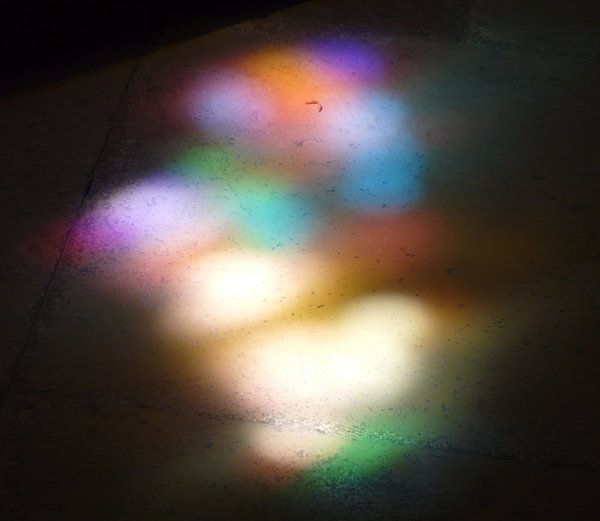
\includegraphics[width=\linewidth]{lichtspiel.jpg}};\end{tcbcliptitle}}]
\lipsum[1]
\end{tcolorbox}
\end{dispExample}
\end{docEnvironment}

\clearpage
\begin{docTcbKey}{clip title}{\colOpt{=true\textbar false}}{default |true|, initially |false|}
  Sets the title to be clipped to the title area.
\begin{dispExample}
\tcbset{enhanced,width=5cm,colframe=red!50!white,coltitle=black,
  colbacktitle=yellow!50!white}

\begin{tcolorbox}[title=\mbox{This is a title which is unbreakable and far too long}]
This is a tcolorbox.
\end{tcolorbox}

\begin{tcolorbox}[title=\mbox{This is a title which is unbreakable and far too long},
  clip title]
This is a tcolorbox.
\end{tcolorbox}
\end{dispExample}
\end{docTcbKey}


\begin{docTcbKey}{clip upper}{\colOpt{=true\textbar false}}{default |true|, initially |false|}
  Sets the upper part to be clipped to the interior area.
\begin{dispExample}
\newcommand{\mygraphics}[2][]{%
  \tcbox[enhanced,boxsep=0pt,top=0pt,bottom=0pt,left=0pt,
    right=0pt,boxrule=0.4pt,drop fuzzy shadow,clip upper,
    colback=black!75!white,toptitle=2pt,bottomtitle=2pt,nobeforeafter,
    center title,fonttitle=\small\sffamily,title=\detokenize{#2}]
  {\includegraphics[width=\the\dimexpr(\linewidth-4mm)/2\relax]{#2}}}

\mygraphics{lichtspiel.jpg}\hfill
\mygraphics{Basilica_5.png}
\end{dispExample}
\end{docTcbKey}

\clearpage
The example for \refKey{/tcb/clip upper} sizes the box according to
the dimensions of the picture. To do it the other way around, the watermark
options provide an easy solution.
\begin{dispExample}
\newcommand{\mygraphics}[2][]{%
  \tcbox[enhanced,capture=minipage,boxsep=0pt,top=0pt,bottom=0pt,left=0pt,
    right=0pt,boxrule=0.4pt,drop fuzzy shadow,nobeforeafter,
    colback=black!75!white,toptitle=2pt,bottomtitle=2pt,
    center title,fonttitle=\small\sffamily,title=\detokenize{#2},
    width=(\linewidth-4mm)/2,height=6cm,colbacktitle={black},
    watermark zoom=1.0,watermark graphics={#2}]{}}

\mygraphics{lichtspiel.jpg}\hfill
\mygraphics{Basilica_5.png}
\end{dispExample}


\begin{docTcbKey}{clip lower}{\colOpt{=true\textbar false}}{default |true|, initially |false|}
  Sets the lower part to be clipped to the interior area.
\begin{dispExample}
\tcbset{enhanced,width=5cm,colframe=red!50!black,text and listing}

\begin{tcblisting}{}
Donau\-dampf\-schiff\-fahrts\-ka\-pi\-t\"ans\-m\"ut\-zen\-fran\-sen
\end{tcblisting}

\begin{tcblisting}{clip lower}
Donau\-dampf\-schiff\-fahrts\-ka\-pi\-t\"ans\-m\"ut\-zen\-fran\-sen
\end{tcblisting}
\end{dispExample}
\end{docTcbKey}


\clearpage
\subsection{Border Line Option Keys}\label{subsec:borderline}
The following borderline options are applicable for most skins which
use |tikzpicture| as \refKey{/tcb/graphical environment}.
Therefore, the skin \refSkin{standard} does not support these border lines,
but most other skins, e.\,g.\ \refSkin{enhanced}.

The borderlines are independent from the normal |tcolorbox| rules.
They may be used with or without the \refKey{/tcb/segmentation engine}.

The borderlines are stackable, i.\,e.\ several different border lines can be
used on the same |tcolorbox|. They are drawn \emph{after} the box frame and box
interior and \emph{before} overlays or watermarks.

\begin{marker}
Technically, the normal |tcolorbox| rules result from a \tikzname\  \emph{filling}
process. The border lines are created by a \tikzname\  \emph{drawing} process.
This can be used to apply different effects.
\end{marker}


\begin{docTcbKey}{borderline}{=\marg{width}\marg{offset}\marg{options}}{no default, initially unset}
  Adds a new borderline to the stack of border lines.
  This border line is drawn with the given \meta{width} and gets an
  \meta{offset} computed from the frame outline. A positive \meta{offset} value
  moves the borderline inside the |tcolorbox| and a negative \meta{offset} value
  moves it outside without changing the bounding box.\\
  The border line is drawn along a \tikzname\  path with the given \tikzname\  \meta{options}.
  Note that the \tikzname\  |line width| option should not be used here.\\
  The border lines adapt to the rounded corners of the |tcolorbox|. An inside
  borderline will switch to sharp corners if necessary, an outside borderline will
  always be rounded except for \refKey{/tcb/sharp corners}.
\begin{dispExample}
\begin{tcolorbox}[enhanced,title=Rounded corners,fonttitle=\bfseries,boxsep=5pt,
  arc=8pt,
  borderline={0.5pt}{0pt}{red},
  borderline={0.5pt}{5pt}{blue,dotted},
  borderline={0.5pt}{-5pt}{green} ]
This is a tcolorbox.
\end{tcolorbox}
\bigskip
\begin{tcolorbox}[enhanced,title=Sharp corners,fonttitle=\bfseries,boxsep=5pt,
  arc=8pt,sharp corners=downhill,
  borderline={0.5pt}{0pt}{red},
  borderline={0.5pt}{5pt}{blue,dotted},
  borderline={0.5pt}{-5pt}{green} ]
This is a tcolorbox.
\end{tcolorbox}
\end{dispExample}

\begin{dispExample}
% \usepackage{lipsum}
\begin{tcolorbox}[enhanced,arc=3mm,boxrule=1.5mm,boxsep=1.5mm,
  colback=yellow!20!white,
  colframe=blue,
  borderline={1mm}{1mm}{white},
  borderline={1mm}{2mm}{red} ]
  \lipsum[1]
\end{tcolorbox}
\end{dispExample}


\begin{dispExample}
% \usepackage{lipsum}
\begin{tcolorbox}[enhanced,arc=3mm,boxrule=1.5mm,
  frame hidden,colback=blue!10!white,
  borderline={1mm}{0mm}{blue,dotted} ]
  \lipsum[2]
\end{tcolorbox}
\end{dispExample}


\begin{dispExample}
% \usepackage{lipsum}
\begin{tcolorbox}[enhanced,skin=enhancedmiddle,
  frame hidden,interior hidden,top=0mm,bottom=0mm,boxsep=0mm,
  borderline={0.75mm}{0mm}{red},
  borderline={0.75mm}{0.75mm}{red!50!yellow},
  borderline={0.75mm}{1.5mm}{yellow}, ]
  \lipsum[3]
\end{tcolorbox}
\end{dispExample}

\begin{dispExample}
% \usepackage{lipsum}
\newtcolorbox{mygreenbox}[2][]{%
  enhanced,width=\linewidth-6pt,
  enlarge top by=3pt,enlarge bottom by=3pt,
  enlarge left by=3pt,enlarge right by=3pt,
  title={#2},frame hidden,boxrule=0pt,top=1mm,bottom=1mm,
  colframe=green!30!black, colbacktitle=green!50!yellow,
  coltitle=black, colback=green!25!white,
  borderline={0.5pt}{-0.5pt}{green!75!blue},
  borderline={1pt}{-3pt}{green!50!blue},#1}

\begin{mygreenbox}{My title}
  \lipsum[4]
\end{mygreenbox}
\end{dispExample}
\end{docTcbKey}


\begin{docTcbKey}{no borderline}{}{no default, initially set}
  Removes all borderlines if set before.
\end{docTcbKey}


\begin{docTcbKey}{show bounding box}{\colOpt{=\meta{color}}}{default |red|, initially unset}
  Displays the bounding box borderline of a |tcolorbox|.
  Its intended use is debugging and fine tuning.
  It should not be part of a final document.
  The optional \meta{color} is the base color for the bounding box
  borderline.
\begin{dispExample}
\tcbset{enhanced,nobeforeafter,width=4cm,fonttitle=\bfseries}

\begin{tcolorbox}[show bounding box,title=Normal]
This is a tcolorbox.
\end{tcolorbox}%
\begin{tcolorbox}[show bounding box=blue,title=Shadow,drop fuzzy shadow]
This is a tcolorbox.
\end{tcolorbox}%
\begin{tcolorbox}[show bounding box=green,title=Enlarged,drop fuzzy shadow,
  enlarge by=2mm]
This is a tcolorbox.
\end{tcolorbox}
\end{dispExample}
\end{docTcbKey}

\clearpage

\begin{marker}
The following \emph{partial} borderlines act slightly different from the
complete borderlines described before. They ignore rounded corner settings,
their length is not modified by their \meta{offset}, they ignore skin settings
but adapt to breakable boxes.
\end{marker}

\begin{docTcbKey}[][doc new=2014-10-20]{borderline north}{=\marg{width}\marg{offset}\marg{options}}{no default, initially unset}
  Adds a new borderline with the given \meta{width} to the
  north of the |tcolorbox|.
  A positive \meta{offset} value
  moves the borderline inside the |tcolorbox| and a negative \meta{offset} value
  moves it outside without changing the bounding box.
\begin{dispExample*}{sbs,lefthand ratio=0.6}
\begin{tcolorbox}[enhanced,
  borderline north={2pt}{-2pt}{red}]
  This is a \textbf{tcolorbox}.
\end{tcolorbox}
\end{dispExample*}
\end{docTcbKey}

\begin{docTcbKey}[][doc new=2014-10-20]{borderline south}{=\marg{width}\marg{offset}\marg{options}}{no default, initially unset}
  Adds a new borderline with the given \meta{width} to the
  south of the |tcolorbox|.
  A positive \meta{offset} value
  moves the borderline inside the |tcolorbox| and a negative \meta{offset} value
  moves it outside without changing the bounding box.
\begin{dispExample*}{sbs,lefthand ratio=0.6}
\begin{tcolorbox}[enhanced,
  borderline south={2pt}{-2pt}{red}]
  This is a \textbf{tcolorbox}.
\end{tcolorbox}
\end{dispExample*}
\end{docTcbKey}

\begin{docTcbKey}[][doc new=2014-10-20]{borderline east}{=\marg{width}\marg{offset}\marg{options}}{no default, initially unset}
  Adds a new borderline with the given \meta{width} to the
  east of the |tcolorbox|.
  A positive \meta{offset} value
  moves the borderline inside the |tcolorbox| and a negative \meta{offset} value
  moves it outside without changing the bounding box.
\begin{dispExample*}{sbs,lefthand ratio=0.6}
\begin{tcolorbox}[enhanced,
  borderline east={2pt}{-2pt}{red}]
  This is a \textbf{tcolorbox}.
\end{tcolorbox}
\end{dispExample*}
\end{docTcbKey}

\begin{docTcbKey}[][doc new=2014-10-20]{borderline west}{=\marg{width}\marg{offset}\marg{options}}{no default, initially unset}
  Adds a new borderline with the given \meta{width} to the
  west of the |tcolorbox|.
  A positive \meta{offset} value
  moves the borderline inside the |tcolorbox| and a negative \meta{offset} value
  moves it outside without changing the bounding box.
\begin{dispExample*}{sbs,lefthand ratio=0.6}
\begin{tcolorbox}[enhanced,
  borderline west={2pt}{-2pt}{red}]
  This is a \textbf{tcolorbox}.
\end{tcolorbox}
\end{dispExample*}
\end{docTcbKey}

\clearpage
\begin{docTcbKey}[][doc new=2014-10-20]{borderline horizontal}{=\marg{width}\marg{offset}\marg{options}}{no default, initially unset}
  Adds a new borderline with the given \meta{width} to the
  north and south of the |tcolorbox|.
  A positive \meta{offset} value
  moves the borderlines inside the |tcolorbox| and a negative \meta{offset} value
  moves them outside without changing the bounding box.
\begin{dispExample*}{sbs,lefthand ratio=0.6}
\begin{tcolorbox}[blanker,top=3mm,bottom=3mm,
   borderline horizontal={2pt}{0pt}{red}]
  This is a \textbf{tcolorbox}.
\end{tcolorbox}
\end{dispExample*}
\end{docTcbKey}


\begin{docTcbKey}[][doc new=2014-10-20]{borderline vertical}{=\marg{width}\marg{offset}\marg{options}}{no default, initially unset}
  Adds a new borderline with the given \meta{width} to the
  east and west of the |tcolorbox|.
  A positive \meta{offset} value
  moves the borderlines inside the |tcolorbox| and a negative \meta{offset} value
  moves them outside without changing the bounding box.
\begin{dispExample*}{sbs,lefthand ratio=0.6}
\begin{tcolorbox}[blanker,left=3mm,right=3mm,
   borderline vertical={2pt}{0pt}{red}]
  This is a \textbf{tcolorbox}.\\
  My second line.
\end{tcolorbox}
\end{dispExample*}
\end{docTcbKey}

\begin{dispExample}
\begin{tcolorbox}[enhanced,colback=yellow!10!white,boxrule=0pt,frame hidden,
  borderline north={1mm}{-2mm}{red},
  borderline south={1mm}{-2mm}{blue},
  borderline west={1mm}{-2mm}{green},
  borderline east={1mm}{-2mm}{yellow}]
\lipsum[1]
\end{tcolorbox}
\end{dispExample}

\clearpage
\subsection{Shadow Option Keys}\label{subsec:shadows}
The following shadow options are applicable for most skins which
use |tikzpicture| as \refKey{/tcb/graphical environment}.
Therefore, the skin \refSkin{standard} does not support these shadows,
but most other skins, e.\,g.\ \refSkin{enhanced}.

The shadows are stackable, i.\,e.\ several different shadows can be
used on the same |tcolorbox|. They are drawn \emph{before} the box frame is drawn.

\begin{docTcbKey}{no shadow}{}{no default}
  Removes all shadows if set before.
\end{docTcbKey}


\begin{docTcbKey}{shadow}{=\marg{xshift}\marg{yshift}\marg{offset}\marg{options}}{no default}
  Adds a new shadow to the stack of shadows.
  This shadow is follows the outline of the |tcolorbox| but is shifted by
  \meta{xshift} and \meta{yshift}. The \meta{offset} value is a distance value
  from the frame outline.  A positive \meta{offset} value shrinks the shadow
  and a negative \meta{offset} value enlarges the shadow.
  The shadow is filled along a \tikzname\  path with the given \tikzname\  \meta{options}.\\
  The shadows adapt to the rounded corners of the |tcolorbox|. An shrinked shadow
  will switch to sharp corners if necessary, an enlarged shadow may become
  more rounded depending on several factors. But \refKey{/tcb/sharp corners}
  have sharp shadows.
  \begin{marker}
  Shadows are not considered for the bounding box computation by default.
  Large shadows may be overlaped by the following content. But, the
  bounding box can be adapted if necessary.
  \end{marker}

\begin{dispExample*}{sbs,lefthand ratio=0.6}
\tcbset{enhanced,colback=red!5!white,
  colframe=red!75!black,fonttitle=\bfseries}

\begin{tcolorbox}[title=My own shadow,
  shadow={2mm}{-1mm}{0mm}{black!50!white}]
This is a tcolorbox.
\end{tcolorbox}
\par\bigskip
\begin{tcolorbox}[title=Another shadow,
  shadow={-1mm}{-2mm}{0mm}{fill=blue,
    opacity=0.5}]
This is a tcolorbox.
\end{tcolorbox}
\par\bigskip
\begin{tcolorbox}[title=Double shadow,
  shadow={-1.5mm}{-1.5mm}{0mm}{fill=blue,
    opacity=0.25},
  shadow={1.5mm}{-1.5mm}{0mm}{fill=red,
    opacity=0.25}]
This is a tcolorbox.
\end{tcolorbox}
\par\bigskip
\begin{tcolorbox}[title=Far shadow,
  shadow={5.5mm}{-3.5mm}{2mm}{fill=black,
    opacity=0.25}]
This is a tcolorbox.
\end{tcolorbox}
\par\bigskip\bigskip
\begin{tcolorbox}[title=Halo shadow,
  shadow={0mm}{0mm}{-1.5mm}%
     {fill=yellow!75!red,opacity=0.5}]
This is a tcolorbox.
\end{tcolorbox}
\end{dispExample*}
\end{docTcbKey}

\clearpage
\begin{docTcbKey}{fuzzy shadow}{=\marg{xshift}\marg{yshift}\marg{offset}\marg{step}\marg{options}}{no default}
  Adds a new fuzzy shadow to the stack of shadows. Actually, this option
  adds several shadows which appear like a shadow with a fuzzy border.
  This fuzzy shadow is follows the outline of the |tcolorbox| but is shifted by
  \meta{xshift} and \meta{yshift}. The \meta{offset} value is a distance value
  from the frame outline.  A positive \meta{offset} value shrinks the shadow
  and a negative \meta{offset} value enlarges the shadow.
  The \marg{step} value describes a shrink
  offset used for the combination of the partial shadows.
  The shadow is filled along a \tikzname\  path with the given \tikzname\  \meta{options} but
  any |opacity| value will be ignored.
\begin{dispExample*}{sbs,lefthand ratio=0.6}
\tcbset{enhanced,colback=red!5!white,
  colframe=red!75!black,fonttitle=\bfseries}

\begin{tcolorbox}[title=My own shadow,
  fuzzy shadow={2mm}{-1mm}{0mm}{0.1mm}%
               {black!50!white}]
This is a tcolorbox.
\end{tcolorbox}
\par\bigskip
\begin{tcolorbox}[title=Another shadow,
  fuzzy shadow={-1mm}{-2mm}{0mm}{0.2mm}%
               {fill=blue}]
This is a tcolorbox.
\end{tcolorbox}
\par\bigskip
\begin{tcolorbox}[title=Double shadow,
  fuzzy shadow={-1.5mm}{-1.5mm}{0mm}{0.1mm}%
               {blue},
  fuzzy shadow={1.5mm}{-1.5mm}{0mm}{0.1mm}%
               {red}]
This is a tcolorbox.
\end{tcolorbox}
\par\bigskip
\begin{tcolorbox}[title=Far shadow,
  fuzzy shadow={5.5mm}{-3.5mm}{0mm}{0.3mm}%
               {black}]
This is a tcolorbox.
\end{tcolorbox}
\par\bigskip\bigskip
\begin{tcolorbox}[title=Glow shadow,
  fuzzy shadow={0mm}{0mm}{-1.5mm}{0.15mm}%
               {yellow!75!red}]
This is a tcolorbox.
\end{tcolorbox}
\end{dispExample*}

\begin{dispExample}
\newtcolorbox{mybox}[1][]{enhanced,
  fuzzy shadow={1.0mm}{-1.0mm}{0.12mm}{0mm}{blue!50!white},
  fuzzy shadow={-1.0mm}{-1.0mm}{0.12mm}{0mm}{red!50!white},
  fuzzy shadow={-1.0mm}{1.0mm}{0.12mm}{0mm}{green!50!white},
  fuzzy shadow={1.0mm}{1.0mm}{0.12mm}{0mm}{yellow!50!white},#1
}

\begin{mybox}[title=A multi shadow box]
This is a tcolorbox.
\end{mybox}
\end{dispExample}
\end{docTcbKey}


\clearpage
\begin{docTcbKey}{drop shadow}{\colOpt{=\meta{color}}}{style, default |black!50!white|}
  Adds a new shadow with standard dimensions to the stack of shadows.
  Optionally, the \meta{color} for the shadow can be changed.
\begin{dispExample*}{sbs,lefthand ratio=0.6}
\tcbset{enhanced,colback=red!5!white,
  colframe=red!75!black,fonttitle=\bfseries}

\begin{tcolorbox}[drop shadow]
This is a tcolorbox.
\end{tcolorbox}\par\bigskip
\begin{tcolorbox}[title=Another shadow,
  drop shadow=blue]
This is a tcolorbox.
\end{tcolorbox}
\end{dispExample*}
\end{docTcbKey}




\begin{docTcbKey}{drop fuzzy shadow}{\colOpt{=\meta{color}}}{style, default |black!50!white|}
  Adds a new fuzzy shadow with standard dimensions to the stack of shadows.
  Optionally, the \meta{color} for the shadow can be changed.
\begin{dispExample*}{sbs,lefthand ratio=0.6}
\tcbset{enhanced,colback=red!5!white,
  colframe=red!75!black,fonttitle=\bfseries}

\begin{tcolorbox}[drop fuzzy shadow]
This is a tcolorbox.
\end{tcolorbox}\par\bigskip
\begin{tcolorbox}[title=Another shadow,
  drop fuzzy shadow=blue]
This is a tcolorbox.
\end{tcolorbox}
\end{dispExample*}
\end{docTcbKey}


\begin{docTcbKey}{drop midday shadow}{\colOpt{=\meta{color}}}{style, default |black!50!white|}
  Adds a new shadow with standard dimensions to the stack of shadows.
  Optionally, the \meta{color} for the shadow can be changed.
\begin{dispExample*}{sbs,lefthand ratio=0.6}
\tcbset{enhanced,colback=red!5!white,
  colframe=red!75!black,fonttitle=\bfseries}

\begin{tcolorbox}[drop midday shadow]
This is a tcolorbox.
\end{tcolorbox}\par\bigskip
\begin{tcolorbox}[title=Another shadow,
  drop midday shadow=blue]
This is a tcolorbox.
\end{tcolorbox}
\end{dispExample*}
\end{docTcbKey}

\enlargethispage*{2cm}
\begin{docTcbKey}{drop fuzzy midday shadow}{\colOpt{=\meta{color}}}{style, default |black!50!white|}
  Adds a new fuzzy shadow with standard dimensions to the stack of shadows.
  Optionally, the \meta{color} for the shadow can be changed.
\begin{dispExample*}{sbs,lefthand ratio=0.6}
\tcbset{enhanced,colback=red!5!white,
  colframe=red!75!black,fonttitle=\bfseries}

\begin{tcolorbox}[drop fuzzy midday shadow]
This is a tcolorbox.
\end{tcolorbox}\par\bigskip
\begin{tcolorbox}[title=Another shadow,
  drop fuzzy midday shadow=blue]
This is a tcolorbox.
\end{tcolorbox}
\end{dispExample*}
\end{docTcbKey}


\clearpage
\begin{docTcbKey}{halo}{\colOpt{=\meta{size} \texttt{with} \meta{color}}}{style, default |0.9mm with yellow|}
  Adds a new halo shadow with the given \meta{color}
  which overlaps the colorbox an all sides by \meta{size}.
\begin{dispExample*}{sbs,lefthand ratio=0.6}
\tcbset{enhanced,colback=red!5!white,
  colframe=red!75!black,fonttitle=\bfseries}

\begin{tcolorbox}[title=My own halo,halo]
This is a tcolorbox.
\end{tcolorbox}
\par\bigskip\bigskip
\begin{tcolorbox}[title=Another halo,
  halo=2mm with green]
This is a tcolorbox.
\end{tcolorbox}
\end{dispExample*}
\end{docTcbKey}


\begin{docTcbKey}{fuzzy halo}{\colOpt{=\meta{size} \texttt{with} \meta{color}}}{style, default |0.9mm with yellow|}
  Adds a new fuzzy halo shadow with the given \meta{color}
  which overlaps the colorbox an all sides by \meta{size} plus |0.48mm|.
\begin{dispExample*}{sbs,lefthand ratio=0.6}
\tcbset{enhanced,colback=red!5!white,
  colframe=red!75!black,fonttitle=\bfseries}

\begin{tcolorbox}[title=My own halo,fuzzy halo]
This is a tcolorbox.
\end{tcolorbox}
\par\bigskip\bigskip
\begin{tcolorbox}[title=Another halo,
  fuzzy halo=2mm with green]
This is a tcolorbox.
\end{tcolorbox}
\end{dispExample*}

\begin{dispExample}
\begin{tcolorbox}[blank,enhanced jigsaw,boxsep=2pt,arc=2pt,
  fuzzy halo=2mm with red!50!white,
  fuzzy halo=1mm with white]
\lipsum[1]
\end{tcolorbox}
\end{dispExample}
\end{docTcbKey}


\clearpage
For all following shadows, the optionally given \meta{color} for the shadow can be changed
equivalent to the preceding examples.

\begin{docTcbKey}{drop shadow southeast}{\colOpt{=\meta{color}}}{style, default |black!50!white|}
  Adds a new shadow with standard dimensions to the stack of shadows.
  This shadow is identical to \refKey{/tcb/drop shadow}.
\begin{dispExample*}{sbs,lefthand ratio=0.7}
\begin{tcolorbox}[drop shadow southeast,
  enhanced,colback=red!5!white,colframe=red!75!black]
  This is a tcolorbox.
\end{tcolorbox}
\end{dispExample*}
\end{docTcbKey}%

\begin{docTcbKey}{drop shadow south}{\colOpt{=\meta{color}}}{style, default |black!50!white|}
  Adds a new shadow with standard dimensions to the stack of shadows.
  This shadow is identical to \refKey{/tcb/drop midday shadow}.
\begin{dispExample*}{sbs,lefthand ratio=0.7}
\begin{tcolorbox}[drop shadow south,
  enhanced,colback=red!5!white,colframe=red!75!black]
  This is a tcolorbox.
\end{tcolorbox}
\end{dispExample*}
\end{docTcbKey}%

\begin{docTcbKey}{drop shadow southwest}{\colOpt{=\meta{color}}}{style, default |black!50!white|}
  Adds a new shadow with standard dimensions to the stack of shadows.
\begin{dispExample*}{sbs,lefthand ratio=0.7}
\begin{tcolorbox}[drop shadow southwest,
  enhanced,colback=red!5!white,colframe=red!75!black]
  This is a tcolorbox.
\end{tcolorbox}
\end{dispExample*}
\end{docTcbKey}%

\begin{docTcbKey}{drop shadow west}{\colOpt{=\meta{color}}}{style, default |black!50!white|}
  Adds a new shadow with standard dimensions to the stack of shadows.
\begin{dispExample*}{sbs,lefthand ratio=0.7}
\begin{tcolorbox}[drop shadow west,
  enhanced,colback=red!5!white,colframe=red!75!black]
  This is a tcolorbox.
\end{tcolorbox}
\end{dispExample*}
\end{docTcbKey}%

\begin{docTcbKey}{drop shadow northwest}{\colOpt{=\meta{color}}}{style, default |black!50!white|}
  Adds a new shadow with standard dimensions to the stack of shadows.
\begin{dispExample*}{sbs,lefthand ratio=0.7}
\begin{tcolorbox}[drop shadow northwest,
  enhanced,colback=red!5!white,colframe=red!75!black]
  This is a tcolorbox.
\end{tcolorbox}
\end{dispExample*}
\end{docTcbKey}%

\begin{docTcbKey}{drop shadow north}{\colOpt{=\meta{color}}}{style, default |black!50!white|}
  Adds a new shadow with standard dimensions to the stack of shadows.
\begin{dispExample*}{sbs,lefthand ratio=0.7}
\begin{tcolorbox}[drop shadow north,
  enhanced,colback=red!5!white,colframe=red!75!black]
  This is a tcolorbox.
\end{tcolorbox}
\end{dispExample*}
\end{docTcbKey}%

\clearpage
\begin{docTcbKey}{drop shadow northeast}{\colOpt{=\meta{color}}}{style, default |black!50!white|}
  Adds a new shadow with standard dimensions to the stack of shadows.
\begin{dispExample*}{sbs,lefthand ratio=0.7}
\begin{tcolorbox}[drop shadow northeast,
  enhanced,colback=red!5!white,colframe=red!75!black]
  This is a tcolorbox.
\end{tcolorbox}
\end{dispExample*}
\end{docTcbKey}%

\begin{docTcbKey}{drop shadow east}{\colOpt{=\meta{color}}}{style, default |black!50!white|}
  Adds a new shadow with standard dimensions to the stack of shadows.
\begin{dispExample*}{sbs,lefthand ratio=0.7}
\begin{tcolorbox}[drop shadow east,
  enhanced,colback=red!5!white,colframe=red!75!black]
  This is a tcolorbox.
\end{tcolorbox}
\end{dispExample*}
\end{docTcbKey}%


\begin{docTcbKey}{drop fuzzy shadow southeast}{\colOpt{=\meta{color}}}{style, default |black!50!white|}
  Adds a new fuzzy shadow with standard dimensions to the stack of shadows.
  This shadow is identical to \refKey{/tcb/drop fuzzy shadow}.
\begin{dispExample*}{sbs,lefthand ratio=0.7}
\begin{tcolorbox}[drop fuzzy shadow southeast,
  enhanced,colback=red!5!white,colframe=red!75!black]
  This is a tcolorbox.
\end{tcolorbox}
\end{dispExample*}
\end{docTcbKey}%

\begin{docTcbKey}{drop fuzzy shadow south}{\colOpt{=\meta{color}}}{style, default |black!50!white|}
  Adds a new fuzzy shadow with standard dimensions to the stack of shadows.
  This shadow is identical to \refKey{/tcb/drop fuzzy midday shadow}.
\begin{dispExample*}{sbs,lefthand ratio=0.7}
\begin{tcolorbox}[drop fuzzy shadow south,
  enhanced,colback=red!5!white,colframe=red!75!black]
  This is a tcolorbox.
\end{tcolorbox}
\end{dispExample*}
\end{docTcbKey}%

\begin{docTcbKey}{drop fuzzy shadow southwest}{\colOpt{=\meta{color}}}{style, default |black!50!white|}
  Adds a new fuzzy shadow with standard dimensions to the stack of shadows.
\begin{dispExample*}{sbs,lefthand ratio=0.7}
\begin{tcolorbox}[drop fuzzy shadow southwest,
  enhanced,colback=red!5!white,colframe=red!75!black]
  This is a tcolorbox.
\end{tcolorbox}
\end{dispExample*}
\end{docTcbKey}%

\begin{docTcbKey}{drop fuzzy shadow west}{\colOpt{=\meta{color}}}{style, default |black!50!white|}
  Adds a new fuzzy shadow with standard dimensions to the stack of shadows.
\begin{dispExample*}{sbs,lefthand ratio=0.7}
\begin{tcolorbox}[drop fuzzy shadow west,
  enhanced,colback=red!5!white,colframe=red!75!black]
  This is a tcolorbox.
\end{tcolorbox}
\end{dispExample*}
\end{docTcbKey}%

\clearpage
\begin{docTcbKey}{drop fuzzy shadow northwest}{\colOpt{=\meta{color}}}{style, default |black!50!white|}
  Adds a new fuzzy shadow with standard dimensions to the stack of shadows.
\begin{dispExample*}{sbs,lefthand ratio=0.7}
\begin{tcolorbox}[drop fuzzy shadow northwest,
  enhanced,colback=red!5!white,colframe=red!75!black]
  This is a tcolorbox.
\end{tcolorbox}
\end{dispExample*}
\end{docTcbKey}%

\begin{docTcbKey}{drop fuzzy shadow north}{\colOpt{=\meta{color}}}{style, default |black!50!white|}
  Adds a new fuzzy shadow with standard dimensions to the stack of shadows.
\begin{dispExample*}{sbs,lefthand ratio=0.7}
\begin{tcolorbox}[drop fuzzy shadow north,
  enhanced,colback=red!5!white,colframe=red!75!black]
  This is a tcolorbox.
\end{tcolorbox}
\end{dispExample*}
\end{docTcbKey}%

\begin{docTcbKey}{drop fuzzy shadow northeast}{\colOpt{=\meta{color}}}{style, default |black!50!white|}
  Adds a new fuzzy shadow with standard dimensions to the stack of shadows.
\begin{dispExample*}{sbs,lefthand ratio=0.7}
\begin{tcolorbox}[drop fuzzy shadow northeast,
  enhanced,colback=red!5!white,colframe=red!75!black]
  This is a tcolorbox.
\end{tcolorbox}
\end{dispExample*}
\end{docTcbKey}%

\begin{docTcbKey}{drop fuzzy shadow east}{\colOpt{=\meta{color}}}{style, default |black!50!white|}
  Adds a new fuzzy shadow with standard dimensions to the stack of shadows.
\begin{dispExample*}{sbs,lefthand ratio=0.7}
\begin{tcolorbox}[drop fuzzy shadow east,
  enhanced,colback=red!5!white,colframe=red!75!black]
  This is a tcolorbox.
\end{tcolorbox}
\end{dispExample*}
\end{docTcbKey}%


\clearpage
\begin{docTcbKey}{lifted shadow}{=\marg{xshift}\marg{yshift}\marg{bend}\marg{step}\marg{options}}{no default}
  Adds a new lifted shadow to the stack of shadows. Actually, this option
  adds several shadows which appear like a shadow with a fuzzy border.
  This lifted shadow is follows the outline of the |tcolorbox| but is shifted by
  \meta{xshift} and \meta{yshift} on the lower left corner and by
  $-$\meta{xshift} and \meta{yshift} on the lower right corner.
  Additionally, there is a \meta{bend} in the middle.
  The \marg{step} value describes a shrink
  offset used for the combination of the partial shadows.
  The shadow is filled along a \tikzname\  path with the given \tikzname\  \meta{options} but
  any |opacity| value will be ignored.
\begin{dispExample*}{sbs,lefthand ratio=0.6}
\tcbset{enhanced,colback=red!5!white,
  boxrule=0.1pt,
  colframe=red!75!black,fonttitle=\bfseries}

\begin{tcolorbox}[title=My own shadow,
  lifted shadow={1mm}{-2mm}{3mm}{0.1mm}%
               {black!50!white}]
This is a tcolorbox.
\end{tcolorbox}
\end{dispExample*}
\end{docTcbKey}

\begin{docTcbKey}{drop lifted shadow}{\colOpt{=\meta{color}}}{style, default |black!50!white|}
  Adds a new lifted shadow with standard dimensions to the stack of shadows.
  Optionally, the \meta{color} for the shadow can be changed.
\begin{dispExample*}{sbs,lefthand ratio=0.6}
\tcbset{enhanced,colback=red!5!white,
  boxrule=0.4pt,sharp corners,
  colframe=red!75!black,fonttitle=\bfseries}

\begin{tcolorbox}[drop lifted shadow]
This is a tcolorbox.
\end{tcolorbox}\par\bigskip
\begin{tcolorbox}[title=Another shadow,
  drop lifted shadow=blue]
This is a tcolorbox.
\end{tcolorbox}
\end{dispExample*}
\end{docTcbKey}


\begin{docTcbKey}{drop small lifted shadow}{\colOpt{=\meta{color}}}{style, default |black!50!white|}
  Adds a new small lifted shadow with standard dimensions to the stack of shadows.
  Optionally, the \meta{color} for the shadow can be changed.
\begin{dispExample*}{sbs,lefthand ratio=0.6}
\tcbset{enhanced,colback=red!5!white,
  boxrule=0.4pt,sharp corners,
  colframe=red!75!black,fonttitle=\bfseries}

\tcbox[drop small lifted shadow,size=fbox]
  {This is a tcolorbox.}
\par\bigskip
\begin{tcolorbox}[title=Another shadow,
  drop small lifted shadow=black]
This is a tcolorbox.
\end{tcolorbox}
\end{dispExample*}
\end{docTcbKey}


\clearpage
\begin{docTcbKey}{drop large lifted shadow}{\colOpt{=\meta{color}}}{style, default |black!50!white|}
  Adds a new large lifted shadow with standard dimensions to the stack of shadows.
  Optionally, the \meta{color} for the shadow can be changed.
\begin{dispExample*}{sbs,lefthand ratio=0.6}
\tcbset{enhanced,colback=red!5!white,
  colframe=red!75!black,fonttitle=\bfseries}

\begin{tcolorbox}[drop large lifted shadow]
This is a tcolorbox.
\end{tcolorbox}\par\bigskip
\begin{tcolorbox}[title=Another shadow,
  drop large lifted shadow=blue]
This is a tcolorbox.
\end{tcolorbox}
\end{dispExample*}
\end{docTcbKey}



\clearpage
\subsection{\tikzname\  Picture Option Keys}\label{subsec:tikzpicture}
The following general options are applicable for skins which
use |tikzpicture| as \refKey{/tcb/graphical environment}.
Therefore, the skin \refSkin{standard} does not support these options,
but most other skins, e.\,g.\ \refSkin{enhanced}.


\begin{docTcbKey}{tikz}{=\meta{tikz option list}}{no default, initially empty}
  Adds the given \meta{tikz option list} to the main |tikzpicture| environment
  used to draw the color box, see \cite{tantau:2013a}. If this option is
  applied a second time, the new \meta{tikz option list} is appended to the
  current option list.
\begin{dispExample*}{sbs,lefthand ratio=0.66,
  segmentation style={pattern=crosshatch dots light steel blue}}
\tcbset{enhanced,colback=red!5!white,
  colframe=red!75!black,fonttitle=\bfseries}

\begin{tcolorbox}[title=Transparent box,
  tikz={opacity=0.5,transparency group}]
This is a tcolorbox.
\end{tcolorbox}
\end{dispExample*}

\begin{dispExample*}{sbs,lefthand ratio=0.66}
\tcbset{enhanced,colback=red!5!white,
  colframe=red!75!black,fonttitle=\bfseries,
  fontupper=\bfseries\Huge,
  center title,center upper}

\begin{tcolorbox}[title=Rotated box,
  tikz={rotate=30}]
Sold!
\end{tcolorbox}
\end{dispExample*}

\end{docTcbKey}


\begin{docTcbKey}{tikz reset}{}{initially set}
  Removes all options given by \refKey{/tcb/tikz}.
\end{docTcbKey}


\begin{docTcbKey}{at begin tikz}{=\meta{tikz code}}{no default, initially empty}
  The given \meta{tikz code} is executed at the beginning of the |tikzpicture| environment
  after the \tikzname\  option |execute at begin picture| was applied.
  If this option is applied a second time, the new \meta{tikz code} is appended to the current code.
\end{docTcbKey}


\begin{docTcbKey}{at begin tikz reset}{}{initially set}
  Removes all code given by \refKey{/tcb/at begin tikz}.
\end{docTcbKey}


\begin{docTcbKey}{at end tikz}{=\meta{tikz code}}{no default, initially empty}
  The given \meta{tikz code} is executed at the ending of the |tikzpicture| environment
  before the \tikzname\  option |execute at end picture| was applied.
  If this option is applied a second time, the new \meta{tikz code} is appended to the current code.
\end{docTcbKey}


\begin{docTcbKey}{at end tikz reset}{}{initially set}
  Removes all code given by \refKey{/tcb/at end tikz}.
\end{docTcbKey}


\clearpage
\begin{docTcbKey}{rotate}{=\meta{angle}}{no default, initially unset}
  Rotates the |tcolorbox| by the given \meta{angle}. Note that this is
  a \tikzname\  coordinate transformation i.e. not all graphical elements like shadings
  will really be rotated.
\begin{dispExample*}{sbs,lefthand ratio=0.66}
\tcbset{enhanced,colback=red!5!white,
  colframe=red!75!black,fonttitle=\bfseries}

\begin{tcolorbox}[title=Rotated box,rotate=30]
This is a tcolorbox.
\end{tcolorbox}
\end{dispExample*}
\end{docTcbKey}

\begin{docTcbKey}{scale}{=\meta{fraction}}{no default, initially unset}
  Scales the |tcolorbox| by the given \meta{fraction}. Note that this is
  a \tikzname\  coordinate transformation i.e. not all graphical elements like line widths
  will really be scaled.
\begin{dispExample*}{sbs,lefthand ratio=0.66}
\tcbset{enhanced,colback=red!5!white,
  colframe=red!75!black,fonttitle=\bfseries}

\begin{tcolorbox}[title=Scaled box,scale=0.5]
This is a tcolorbox.
\end{tcolorbox}
\begin{tcolorbox}[title=Scaled box,scale=1.25]
This is a tcolorbox.
\end{tcolorbox}
\end{dispExample*}
\end{docTcbKey}


\begin{docTcbKey}{remember}{}{style, initially unset}
  Shortcut for |tikz={remember picture}|. This allows one to reference nodes
  in other \tikzname\  pictures.
\begin{dispExample}
\begin{tcolorbox}[enhanced,remember,colback=red!5!white,colframe=red!75!black,
  fonttitle=\bfseries,title=The four corners of a paper,
  overlay={\draw[red!50!white,line width=1mm,opacity=0.5,shorten >=3mm]
    (frame.north west) edge[->] (current page.north west)
    (frame.north east) edge[->] (current page.north east)
    (frame.south west) edge[->] (current page.south west)
    (frame.south east) edge[->] (current page.south east);}]
This is a tcolorbox.
\end{tcolorbox}
\end{dispExample}
\end{docTcbKey}

\clearpage
\tcbinterruptdraftmode%
\begin{docTcbKey}{remember as}{=\meta{name}}{style, no default, initially unset}
  The |frame| node will be remembered by the given \meta{name} to be referenced
  in other \tikzname\  pictures.
\begin{dispExample}
% \usepackage{lipsum}
\newtcolorbox{mybox}[1][]{enhanced,colframe=blue!75!black,colback=blue!10!white,
  fonttitle=\bfseries,#1}

\begin{mybox}[title=First Box,nobeforeafter,width=\linewidth/4,remember as=one]
This is a test.
\end{mybox}
\hfill
\begin{mybox}[title=Second Box,nobeforeafter,width=\linewidth/4,remember as=two]
This is a test.
\end{mybox}
\hfill
\begin{mybox}[title=Third Box,nobeforeafter,width=\linewidth/4,remember as=three]
This is a test.
\end{mybox}

\lipsum[2]

\begin{mybox}[title=Fourth Box,remember as=four]
This is a test.
\end{mybox}

\begin{tikzpicture}[overlay,remember picture,line width=1mm,draw=red!75!black]
  \draw[->] (one.east) to[bend right] node[above] {A} (two.west);
  \draw[->] (two.east) to[bend left] node[above] {B} (three.west);
  \draw[->] (three.east) to[bend left=90] node[right] {C} (four.east);
  \draw[->] (four.west) to[bend left=90] node[left] {D} (one.west);
\end{tikzpicture}
\end{dispExample}
\end{docTcbKey}
\tcbcontinuedraftmode%


\clearpage
\subsection{Underlay Option Keys}\label{subsec:skinunderlay}

Underlays are quite similar to overlays described in \Vref{subsec:overlays}.
Underlays are drawn \emph{after} the frame and interior are
drawn and \emph{before} overlays and the text content is drawn; see
\Vref{subsec:tcolorboxdrawing} for the general drawing scheme.

The differences between underlays and overlays are:
\begin{itemize}
\item Underlays are not applicable for the skins
  \refSkin{standard} and
  \refSkin{standard jigsaw},
  whereas overlays are applicable also for these skins.
  The skin \refSkin{spartan} supports underlays but no overlays.
  \begin{marker}
  If an underlay is used with the \refSkin{standard} skin, it is silently ignored.
  \end{marker}
\item Underlays are stackable, i.\,e.\ several different underlays can be
  used on the same |tcolorbox|. Overlays are not stackable by default (but with
  some help of the library \mylib{hooks}).
\item Boxed titles are implemented with underlays (\Vref{subsec:skinboxedtitle}),
  watermarks are implemented with overlays (\Vref{subsec:watermarks}).
\end{itemize}


\begin{docTcbKey}{underlay}{=\meta{graphical code}}{no default, initially unset}
  Adds \meta{graphical code} to the box drawing process. This \meta{graphical code}
  is drawn \emph{after} the frame and interior and \emph{before} the text content.
\begin{dispExample}
\newtcolorbox{mybox}[1][]{enhanced,colback=red!5!white,
  colbacktitle=red!85!black!50!white,
  colframe=red!75!black,fonttitle=\bfseries,watermark color=yellow!50!white,
  underlay={\begin{tcbclipinterior}
    \draw[red!40!white,line width=1cm] (interior.south west)--(interior.north east);
    \end{tcbclipinterior}},
  attach boxed title to top center={yshift=-2mm},#1}

\begin{mybox}[title=My box,watermark text=My Watermark]
\lipsum[2]
\end{mybox}
\end{dispExample}
\end{docTcbKey}


\begin{docTcbKey}{no underlay}{}{style, no default, initially set}
  Removes the underlay if set before.
\end{docTcbKey}

\clearpage
\begin{docTcbKey}{underlay broken}{=\meta{graphical code}}{no default, initially unset}
  If the box is set to be \refKey{/tcb/breakable} and \emph{is} broken actually,
  then the \meta{graphical code} is added to the box drawing process.
  \refKey{/tcb/underlay} overwrites this key.
\end{docTcbKey}

\begin{docTcbKey}{underlay unbroken}{=\meta{graphical code}}{no default, initially unset}
  If the box is set to be \refKey{/tcb/breakable} but \emph{is not} broken actually
  or if the box is set to be \refKey{/tcb/unbreakable},
  then the \meta{graphical code} is added to the box drawing process.
  \refKey{/tcb/underlay} overwrites this key.
\end{docTcbKey}

\begin{docTcbKey}{no underlay unbroken}{}{style, no default, initially set}
  Removes the unbroken underlay if set before.
\end{docTcbKey}

\begin{docTcbKey}{underlay first}{=\meta{graphical code}}{no default, initially unset}
  If the box is set to be \refKey{/tcb/breakable} and \emph{is} broken actually,
  then the \meta{graphical code} is added to the box drawing process for
  the \emph{first} part of the break sequence.
  \refKey{/tcb/underlay} overwrites this key.
\end{docTcbKey}

\begin{docTcbKey}{no underlay first}{}{style, no default, initially set}
  Removes the first underlay if set before.
\end{docTcbKey}

\begin{docTcbKey}{underlay middle}{=\meta{graphical code}}{no default, initially unset}
  If the box is set to be \refKey{/tcb/breakable} and \emph{is} broken actually,
  then the \meta{graphical code} is added to the box drawing process for
  the \emph{middle} parts (if any) of the break sequence.
  \refKey{/tcb/underlay} overwrites this key.
\end{docTcbKey}

\begin{docTcbKey}{no underlay middle}{}{style, no default, initially set}
  Removes the middle underlay if set before.
\end{docTcbKey}

\begin{docTcbKey}{underlay last}{=\meta{graphical code}}{no default, initially unset}
  If the box is set to be \refKey{/tcb/breakable} and \emph{is} broken actually,
  then the \meta{graphical code} is added to the box drawing process for
  the \emph{last} part of the break sequence.
  \refKey{/tcb/underlay} overwrites this key.
\end{docTcbKey}

\begin{docTcbKey}{no underlay last}{}{style, no default, initially set}
  Removes the last underlay if set before.
\end{docTcbKey}

\begin{docTcbKey}{underlay boxed title}{=\meta{graphical code}}{no default, initially unset}
  If the box has a \emph{boxed title}, see \Vref{subsec:skinboxedtitle},
  then the \meta{graphical code} is added to the box drawing process
  \emph{before} the boxed title is drawn.
\end{docTcbKey}

\begin{docTcbKey}{no underlay boxed title}{}{style, no default, initially set}
  Removes the boxed title underlay if set before.
\end{docTcbKey}

\begin{docTcbKey}{underlay unbroken and first}{=\meta{graphical code}}{no default, initially unset}
  This is an abbreviation for setting
  \refKey{/tcb/underlay unbroken} and
  \refKey{/tcb/underlay first} together.
  \refKey{/tcb/underlay} overwrites this key.
\end{docTcbKey}

\begin{docTcbKey}{underlay middle and last}{=\meta{graphical code}}{no default, initially unset}
  This is an abbreviation for setting
  \refKey{/tcb/underlay middle} and
  \refKey{/tcb/underlay last} together.
  \refKey{/tcb/underlay} overwrites this key.
\end{docTcbKey}

\begin{docTcbKey}{underlay unbroken and last}{=\meta{graphical code}}{no default, initially unset}
  This is an abbreviation for setting
  \refKey{/tcb/underlay unbroken} and
  \refKey{/tcb/underlay last} together.
  \refKey{/tcb/underlay} overwrites this key.
\end{docTcbKey}

\begin{docTcbKey}[][doc new=2014-09-19]{underlay first and middle}{=\meta{graphical code}}{no default, initially unset}
  This is an abbreviation for setting
  \refKey{/tcb/underlay first} and
  \refKey{/tcb/underlay middle} together.
  \refKey{/tcb/underlay} overwrites this key.
\end{docTcbKey}


\clearpage
\subsection{Finish Option Keys}\label{subsec:skinfinish}

Finishes are quite similar to underlays described in \Vref{subsec:skinunderlay}
and overlays described in \Vref{subsec:overlays}.
Finishes are drawn \emph{after} the text content is drawn; see
\Vref{subsec:tcolorboxdrawing} for the general drawing scheme.
Therefore, a finish will reduce the readability of the text content.

Finishes are intended for special effects like highlights or glosses or text over text.

\begin{itemize}
\item Finishes are only applicable for the skins
  \refSkin{enhanced},
  \refSkin{empty},
  \refSkin{freelance},
  \refSkin{bicolor},
  \refSkin{beamer}, and
  \refSkin{widget}.
  \begin{marker}
  If a finish is used with the \refSkin{standard} skin, it is silently ignored.
  \end{marker}
\item Finishes are stackable, i.\,e.\ several different finishes can be
  used on the same |tcolorbox|.
\end{itemize}

\enlargethispage*{2cm}
\begin{docTcbKey}{finish}{=\meta{graphical code}}{no default, initially unset}
  Adds \meta{graphical code} to the box drawing process. This \meta{graphical code}
  is drawn \emph{after} the text content.
\begin{dispExample}
\newtcolorbox{mybox}[1][]{enhanced,colback=red!5!white,
  colbacktitle=red!85!black!50!white,colframe=red!75!black,fonttitle=\bfseries,
  finish={\begin{tcbclipframe}
    \path[bottom color=black,top color=black!50!white,opacity=0.1]
      (frame.south west) -- (frame.south east) -- (frame.north east) -- cycle;
    \path[top color=white,bottom color=black!50!white,opacity=0.1]
      (frame.south west) -- (frame.north east) -- (frame.north west) -- cycle;
    \end{tcbclipframe}},#1}

\begin{mybox}[title=My box]
\lipsum[2]
\end{mybox}
\end{dispExample}
\begin{dispExample}
\newtcolorbox{mybox}[1][]{enhanced,colback=red!5!white,
  colbacktitle=red!85!black!50!white,colframe=red!75!black,fonttitle=\bfseries,
  finish={\node[draw,fill=white,fill opacity=0.85,inner sep=5mm,
    rounded corners] at (frame.center) {\Huge\bfseries Finish!};},#1}

\begin{mybox}[title=My box]
\lipsum[2]
\end{mybox}
\end{dispExample}
\end{docTcbKey}

\clearpage
\begin{docTcbKey}{no finish}{}{style, no default, initially set}
  Removes the finish if set before.
\end{docTcbKey}


\begin{docTcbKey}{finish broken}{=\meta{graphical code}}{no default, initially unset}
  If the box is set to be \refKey{/tcb/breakable} and \emph{is} broken actually,
  then the \meta{graphical code} is added to the box drawing process.
  \refKey{/tcb/finish} overwrites this key.
\end{docTcbKey}

\begin{docTcbKey}{finish unbroken}{=\meta{graphical code}}{no default, initially unset}
  If the box is set to be \refKey{/tcb/breakable} but \emph{is not} broken actually
  or if the box is set to be \refKey{/tcb/unbreakable},
  then the \meta{graphical code} is added to the box drawing process.
  \refKey{/tcb/finish} overwrites this key.
\end{docTcbKey}

\begin{docTcbKey}{no finish unbroken}{}{style, no default, initially set}
  Removes the unbroken finish if set before.
\end{docTcbKey}

\begin{docTcbKey}{finish first}{=\meta{graphical code}}{no default, initially unset}
  If the box is set to be \refKey{/tcb/breakable} and \emph{is} broken actually,
  then the \meta{graphical code} is added to the box drawing process for
  the \emph{first} part of the break sequence.
  \refKey{/tcb/finish} overwrites this key.
\end{docTcbKey}

\begin{docTcbKey}{no finish first}{}{style, no default, initially set}
  Removes the first finish if set before.
\end{docTcbKey}

\begin{docTcbKey}{finish middle}{=\meta{graphical code}}{no default, initially unset}
  If the box is set to be \refKey{/tcb/breakable} and \emph{is} broken actually,
  then the \meta{graphical code} is added to the box drawing process for
  the \emph{middle} parts (if any) of the break sequence.
  \refKey{/tcb/finish} overwrites this key.
\end{docTcbKey}

\begin{docTcbKey}{no finish middle}{}{style, no default, initially set}
  Removes the middle finish if set before.
\end{docTcbKey}

\begin{docTcbKey}{finish last}{=\meta{graphical code}}{no default, initially unset}
  If the box is set to be \refKey{/tcb/breakable} and \emph{is} broken actually,
  then the \meta{graphical code} is added to the box drawing process for
  the \emph{last} part of the break sequence.
  \refKey{/tcb/finish} overwrites this key.
\end{docTcbKey}

\begin{docTcbKey}{no finish last}{}{style, no default, initially set}
  Removes the last finish if set before.
\end{docTcbKey}

\begin{docTcbKey}{finish unbroken and first}{=\meta{graphical code}}{no default, initially unset}
  This is an abbreviation for setting
  \refKey{/tcb/finish unbroken} and
  \refKey{/tcb/finish first} together.
  \refKey{/tcb/finish} overwrites this key.
\end{docTcbKey}

\begin{docTcbKey}{finish middle and last}{=\meta{graphical code}}{no default, initially unset}
  This is an abbreviation for setting
  \refKey{/tcb/finish middle} and
  \refKey{/tcb/finish last} together.
  \refKey{/tcb/finish} overwrites this key.
\end{docTcbKey}

\begin{docTcbKey}{finish unbroken and last}{=\meta{graphical code}}{no default, initially unset}
  This is an abbreviation for setting
  \refKey{/tcb/finish unbroken} and
  \refKey{/tcb/finish last} together.
  \refKey{/tcb/finish} overwrites this key.
\end{docTcbKey}


\begin{docTcbKey}[][doc new=2014-09-19]{finish first and middle}{=\meta{graphical code}}{no default, initially unset}
  This is an abbreviation for setting
  \refKey{/tcb/finish first} and
  \refKey{/tcb/finish middle} together.
  \refKey{/tcb/finish} overwrites this key.
\end{docTcbKey}


\clearpage
\subsection{Jigsaw Skin Variants}\label{subsec:skinjigsaw}
As described in \Vref{sec:skincorekeys}, a |tcolorbox| is drawn by up to
four \emph{engines}. Typically, the \emph{frame} engine fills the complete box area
with color and the other engines fill certain areas with other colors.
Finally, only the area which you see as \emph{frame} of the box will display
the frame color. For most applications, this is a good approach.

For certain boxes, a more delicate procedure is needed. E.g., if the box should
be translucent, an already painted area cannot be made unpainted. Therefore,
more elaborate frame engines saw holes into the frame where the interior area and
optionally the title area will be painted.
The resulting skins are called \emph{jigsaw} skins. For \refSkin{standard}
and \refSkin{enhanced}, there are variants called \refSkin{standard jigsaw}
and \refSkin{enhanced jigsaw}.


\begin{dispExample}
\newcommand{\ballexample}{\begin{tikzpicture}
  \path[use as bounding box] (0,0.8) rectangle +(0.1,0.1);
  \shadedraw [shading=ball] (0,0) circle (1cm);
  \shadedraw [ball color=red] (3,-2.2) circle (1cm);
\end{tikzpicture}}

\tcbset{enhanced,colback=blue!5!white,
  frame style={left color=red!75!black,right color=red!10!yellow},
  fonttitle=\bfseries }

\ballexample

\begin{tcolorbox}[title=A normal box]
  \lipsum[2]
\end{tcolorbox}

\ballexample

\begin{tcolorbox}[title=A translucent jigsaw box,
  enhanced jigsaw,opacityback=0.35]
  \lipsum[2]
\end{tcolorbox}
\end{dispExample}


\begin{dispExample*}{segmentation style={pattern=crosshatch dots light steel blue}}
\tcbset{enhanced,colback=red!10!white,coltitle=black,
  frame style={left color=red!75!black,right color=red!10!yellow},
  fonttitle=\bfseries,interior hidden,title hidden}

\begin{tcolorbox}[title=A normal box with hidden interior and title]
  This is a tcolorbox.
\end{tcolorbox}

\begin{tcolorbox}[enhanced jigsaw,
  title=A jigsaw box with hidden interior and title]
  This is a tcolorbox.
\end{tcolorbox}
\end{dispExample*}


\begin{dispExample}
\newtcolorbox{mybox}{skin=enhancedmiddle jigsaw,leftrule=5mm,rightrule=5mm,
  boxsep=0mm,top=0mm,bottom=0mm,
  frame style={top color=blue,bottom color=red},interior hidden}

\begin{mybox}
  \lipsum[2]
\end{mybox}
\end{dispExample}


\clearpage
\subsection{Draft Mode}\label{subsec:draftmode}
To reduce the compiliation time while drafting a document, the \emph{draft mode}
can be applied. Basically, it changes all skins to \refSkin{spartan} and
sets the \refKey{/tcb/fit algorithm} to |squeeze|. Especially,
when fuzzy shadows are used, the speedup will be considerable high.

\begin{marker}
It is strongly recommended that the draft mode is \emph{not} used for the final document.
Use \refSkin{spartan} directly, if you want to stay with it. The draft mode
implementation may change in future.
\end{marker}

\begin{marker}
Normally, switching to the draft mode should not alter the geometry of
your document. Since overlays are deactivated, any code placed there
(e.g. counter changes) is not executed anymore! Also, \refKey{/tcb/remember as}
will not have any effect. You may exclude critical code with
\refCom{tcbinterruptdraftmode} / \refCom{tcbcontinuedraftmode}
from converting to draft mode.
\end{marker}


\begin{docCommand}{tcbstartdraftmode}{}
  Any following |tcolorbox| code is put into \emph{draft mode}. All skin
  settings are overruled with \refSkin{spartan}. Overlays, watermarks,
  shadows, borderlines, and rounded corners are deactivated for all |tcolorbox|
  layers.
\end{docCommand}

\begin{docCommand}{tcbstopdraftmode}{}
  The \emph{draft mode} is deactivated for the following code.
\end{docCommand}

\begin{docCommand}{tcbinterruptdraftmode}{}
  If the compilation is in \emph{draft mode}, the \emph{draft mode} is deactivated
  until a following \refCom{tcbcontinuedraftmode} is detected.\par
  If the compilation is not in \emph{draft mode}, nothing happens and a following
  \refCom{tcbcontinuedraftmode} will not start the \emph{draft mode}.
  \begin{marker}
  The pair |\tcbinterruptdraftmode| and |\tcbcontinuedraftmode| cannot
  be used nested.
  \end{marker}
\end{docCommand}

\begin{docCommand}{tcbcontinuedraftmode}{}
  Continues the \emph{draft mode} which was suspended by a preceding
  \refCom{tcbinterruptdraftmode}. Nothing happens, if there was no draft
  mode before \refCom{tcbinterruptdraftmode}.
  \begin{marker}
  Code, which is place between \refCom{tcbinterruptdraftmode} and
  \refCom{tcbcontinuedraftmode} is shielded from \emph{draft mode}.
  \end{marker}
\end{docCommand}

\enlargethispage*{2cm}
\begin{docTcbKey}{draftmode}{\colOpt{=true\textbar false}}{default |true|, initially |false|}
  If set to |true|, the \emph{draft mode} is started.
  If set to |false|, the \emph{draft mode} is stopped.

\begin{dispExample*}{}
\newtcolorbox{mybeamer}[2][]{beamer,colback=Salmon!50!white,
  colframe=FireBrick!75!black,adjusted title={#2},#1}

\begin{mybeamer}{Beamer box}
This box looks like a box provided by the \texttt{beamer} class.
\end{mybeamer}\par\medskip
\begin{mybeamer}[draftmode]{Beamer box}
This box looks like a box provided by the \texttt{beamer} class.
\end{mybeamer}
\end{dispExample*}
\end{docTcbKey}



\clearpage
\tcbset{skintable/.style={colframe=red!50!yellow!50!black,
  colback=red!50!yellow!5!white,coltitle=red!50!yellow!3!white,
  fonttitle=\bfseries,before=\par\smallskip,
  title=Environment and engines for the skin '\texttt{#1}'}}

\subsection{Skin Family 'standard'}\label{subsec:skinstandard}
\begin{marker}Note that the option keys \refKey{/tcb/frame style},
  \refKey{/tcb/interior style},
  \refKey{/tcb/segmentation style}, and
  \refKey{/tcb/title style} are not be applicable to the standard skin.
  Also, watermarks (see Subsection \ref{subsec:watermarks})
  are not usable with the standard skin.
\end{marker}

\begin{docSkin}{standard}
  This is the standard skin from the core package. All drawing engines
  are set to type |standard|. The drawing is based on |pgf| commands and
  does not need the |tikz| package.
\begin{tcolorbox}[skintable=standard]
  \begin{tabbing}
    \refKey{/tcb/interior titled engine}: \=\kill
    \refKey{/tcb/graphical environment}:  \> |pgfpicture|\\ 
    \refKey{/tcb/frame engine}:           \> |standard|\\
    \refKey{/tcb/interior titled engine}: \> |standard|\\ 
    \refKey{/tcb/interior engine}:        \> |standard|\\
    \refKey{/tcb/segmentation engine}:    \> |standard|\\
    \refKey{/tcb/title engine}:           \> |standard|
  \end{tabbing}
\end{tcolorbox}
\end{docSkin}

\begin{docTcbKey}{standard}{}{style, no value}
  This is an abbreviation for setting |skin=standard|.
\end{docTcbKey}

\begin{dispExample}
\begin{tcbraster}[standard,raster equal height,raster columns=4,
    colback=LightGreen,colframe=DarkGreen,colbacktitle=LimeGreen!75!DarkGreen,
    left=1mm,right=1mm,top=1mm,bottom=1mm,middle=1mm]
  \begin{tcolorbox}
    This is my content.
  \end{tcolorbox}
  \begin{tcolorbox}
    This is my content.
    \tcblower
    More content.
  \end{tcolorbox}
  \begin{tcolorbox}[adjusted title=My title]
    This is my content.
  \end{tcolorbox}
  \begin{tcolorbox}[adjusted title=My title]
    This is my content.
    \tcblower
    More content.
  \end{tcolorbox}
\end{tcbraster}
\end{dispExample}


\clearpage

\begin{docSkin}{standard jigsaw}
  This is the standard jigsaw skin from the core package. It differs from
  the skin \refSkin{standard} by its frame engine, see \Vref{subsec:skinjigsaw}.
\begin{tcolorbox}[skintable=standard jigsaw]
  \begin{tabbing}
    \refKey{/tcb/interior titled engine}: \=\kill
    \refKey{/tcb/graphical environment}:  \> |pgfpicture|\\ 
    \refKey{/tcb/frame engine}:           \> |standardjigsaw|\\
    \refKey{/tcb/interior titled engine}: \> |standard|\\ 
    \refKey{/tcb/interior engine}:        \> |standard|\\
    \refKey{/tcb/segmentation engine}:    \> |standard|\\
    \refKey{/tcb/title engine}:           \> |standard|
  \end{tabbing}
\end{tcolorbox}
\end{docSkin}

\begin{docTcbKey}{standard jigsaw}{}{style, no value}
  This is an abbreviation for setting |skin=standard jigsaw|.
\end{docTcbKey}

\begin{dispExample}
\begin{tcbraster}[standard jigsaw,raster equal height,raster columns=4,
    colback=LightGreen,colframe=DarkGreen,colbacktitle=LimeGreen!75!DarkGreen,
    opacityframe=0.5,opacityback=0.5,opacitybacktitle=0.5,
    left=1mm,right=1mm,top=1mm,bottom=1mm,middle=1mm]
  \begin{tcolorbox}
    This is my content.
  \end{tcolorbox}
  \begin{tcolorbox}
    This is my content.
    \tcblower
    More content.
  \end{tcolorbox}
  \begin{tcolorbox}[adjusted title=My title]
    This is my content.
  \end{tcolorbox}
  \begin{tcolorbox}[adjusted title=My title]
    This is my content.
    \tcblower
    More content.
  \end{tcolorbox}
\end{tcbraster}
\end{dispExample}


\clearpage
\subsection{Skin Family 'enhanced'}
\begin{marker}
If you like the standard appearance of a |tcolorbox| but you want to
have some 'enhanced' features, the |enhanced| skin is what you are looking for.
\end{marker}

\begin{docSkin}{enhanced}
  This skin translates the drawing commands of the core package into |tikz|
  path commands. Therefore, it allows all |tikz| high level options for
  these paths and has more flexibility compared to the \refSkin{standard} skin.
  You pay for this with some prolonged compilation time.
  The |tikz| path options can
  be given with the option keys
  \refKey{/tcb/frame style},
  \refKey{/tcb/interior style},
  \refKey{/tcb/segmentation style}, and
  \refKey{/tcb/title style}.
\begin{tcolorbox}[skintable=enhanced]
  \begin{tabbing}
    \refKey{/tcb/interior titled engine}: \=\kill
    \refKey{/tcb/graphical environment}:  \> |tikzpicture|\\ 
    \refKey{/tcb/frame engine}:           \> |path|\\
    \refKey{/tcb/interior titled engine}: \> |path|\\ 
    \refKey{/tcb/interior engine}:        \> |path|\\
    \refKey{/tcb/segmentation engine}:    \> |path|\\
    \refKey{/tcb/title engine}:           \> |path|
  \end{tabbing}
\end{tcolorbox}
\end{docSkin}


\begin{docTcbKey}{enhanced}{}{style, no value}
  This is an abbreviation for setting |skin=enhanced|.
\end{docTcbKey}

\begin{dispExample}
\begin{tcbraster}[enhanced,raster equal height,raster columns=4,
    colback=LightGreen,colframe=DarkGreen,colbacktitle=LimeGreen!75!DarkGreen,
    left=1mm,right=1mm,top=1mm,bottom=1mm,middle=1mm]
  \begin{tcolorbox}
    This is my content.
  \end{tcolorbox}
  \begin{tcolorbox}
    This is my content.
    \tcblower
    More content.
  \end{tcolorbox}
  \begin{tcolorbox}[adjusted title=My title]
    This is my content.
  \end{tcolorbox}
  \begin{tcolorbox}[adjusted title=My title]
    This is my content.
    \tcblower
    More content.
  \end{tcolorbox}
\end{tcbraster}
\end{dispExample}

\begin{dispExample}
% \usetikzlibrary{shadings}         % preamble
\tcbset{skin=enhanced,fonttitle=\bfseries,
  frame style={upper left=blue,upper right=red,lower left=yellow,lower right=green},
  interior style={white,opacity=0.5},
  segmentation style={black,solid,opacity=0.2,line width=1pt}}

\begin{tcolorbox}[title=Nice box in rainbow colors]
  With the 'enhanced' skin, it is quite easy to produce fancy looking effects.
  \tcblower
  Note that this is still a \texttt{tcolorbox}.
\end{tcolorbox}
\end{dispExample}


\begin{dispExample}
% \usetikzlibrary{decorations.pathmorphing} % preamble
\tcbset{skin=enhanced,fonttitle=\bfseries,boxrule=1mm,
  frame style={draw=FireBrick,fill=Salmon},drop fuzzy shadow,
  interior style={draw=FireBrick,top color=Salmon!10,bottom color=Salmon!20},
  segmentation style={draw=FireBrick,solid,decorate,
        decoration={coil,aspect=0,segment length=10.1mm}}}

\begin{tcblisting}{title=A listing box with shadow and some specials}
Of course, skins can be used for listings also.
\begin{equation}
  \int\limits_1^2 \frac{1}{x}~dx = \ln(2).
\end{equation}
\end{tcblisting}
\end{dispExample}


\clearpage


\begin{docTcbKey}{enhanced standard}{}{style, no value}
  For unbreakable boxes, this is identical to using \refKey{/tcb/enhanced}.
  But, for breakable boxes, the \emph{break sequence} is identical to the \refSkin{standard} skin,
  see Section \ref{subsec:breaksequence} from page \pageref{subsec:breaksequence}.
\end{docTcbKey}


\begin{docTcbKey}{blank}{}{style, initially unset}
  This style relies on the skin \refSkin{enhanced}. All drawing operations
  are hidden and all margins are set to |0pt|. See \refKey{/tcb/blanker}
  for switching off the drawing engines.
\begin{dispExample}
\begin{tcolorbox}[blank,watermark text=A blank box]
\lipsum[1]
\end{tcolorbox}
\end{dispExample}
\end{docTcbKey}

\clearpage
\begin{docCommand}{tcbline}{}
  Sometimes, a line is only a line. With \refCom{tcblower} you separate
  the box content into two functional units. |\tcbline| draws only a line
  which looks like the segmentation line between upper and lower part.
  Furthermore, you can use |\tcbline| more than just once.
  |\tcbline| always uses the |path| drawing engine. Therefore,
  the \refKey{/tcb/segmentation style} can be applied.

\begin{dispExample}
\tcbset{enhanced,colframe=blue!50!black,colback=white}

\begin{tcolorbox}[colupper=red!50!black,collower=green!50!black]
\lipsum[1]
\tcbline
\lipsum[2]
\tcblower
\lipsum[3]
\tcbline
\lipsum[4]
\end{tcolorbox}
\end{dispExample}
\end{docCommand}

\begin{docCommand}{tcbline*}{}
  Equivalent to \refCom{tcbline}, but in a breakable box, \refCom{tcbline*}
  is removed if at a page/box break. Also, it is removed at the end
  of a box.
\end{docCommand}

\clearpage
\begin{docSkin}{enhancedfirst}
This is a flavor of \refSkin{enhanced} which is used as a \emph{first} part
in a break sequence for \refSkin{enhanced}.
Nevertheless, this skin can be applied independently.
\begin{tcolorbox}[skintable=enhancedfirst]
  \begin{tabbing}
    \refKey{/tcb/interior titled engine}: \=\kill
    \refKey{/tcb/graphical environment}:  \> |tikzpicture|\\ 
    \refKey{/tcb/frame engine}:           \> |pathfirst|\\
    \refKey{/tcb/interior titled engine}: \> |pathfirst|\\ 
    \refKey{/tcb/interior engine}:        \> |pathfirst|\\
    \refKey{/tcb/segmentation engine}:    \> |path|\\
    \refKey{/tcb/title engine}:           \> |pathfirst|
  \end{tabbing}
\end{tcolorbox}
\end{docSkin}


\begin{dispExample}
\begin{tcbraster}[skin=enhancedfirst,raster equal height,raster columns=4,
    colback=LightGreen,colframe=DarkGreen,colbacktitle=LimeGreen!75!DarkGreen,
    left=1mm,right=1mm,top=1mm,bottom=1mm,middle=1mm]
  \begin{tcolorbox}
    This is my content.
  \end{tcolorbox}
  \begin{tcolorbox}
    This is my content.
    \tcblower
    More content.
  \end{tcolorbox}
  \begin{tcolorbox}[adjusted title=My title]
    This is my content.
  \end{tcolorbox}
  \begin{tcolorbox}[adjusted title=My title]
    This is my content.
    \tcblower
    More content.
  \end{tcolorbox}
\end{tcbraster}
\end{dispExample}



\clearpage
\begin{docSkin}{enhancedmiddle}
This is a flavor of \refSkin{enhanced} which is used as a \emph{middle} part
in a break sequence for \refSkin{enhanced}.
Nevertheless, this skin can be applied independently.
\begin{tcolorbox}[skintable=enhancedmiddle]
  \begin{tabbing}
    \refKey{/tcb/interior titled engine}: \=\kill
    \refKey{/tcb/graphical environment}:  \> |tikzpicture|\\ 
    \refKey{/tcb/frame engine}:           \> |pathmiddle|\\
    \refKey{/tcb/interior titled engine}: \> |pathmiddle|\\ 
    \refKey{/tcb/interior engine}:        \> |pathmiddle|\\
    \refKey{/tcb/segmentation engine}:    \> |path|\\
    \refKey{/tcb/title engine}:           \> |pathmiddle|
  \end{tabbing}
\end{tcolorbox}
\end{docSkin}


\begin{dispExample}
\begin{tcbraster}[skin=enhancedmiddle,raster equal height,raster columns=4,
    colback=LightGreen,colframe=DarkGreen,colbacktitle=LimeGreen!75!DarkGreen,
    left=1mm,right=1mm,top=1mm,bottom=1mm,middle=1mm]
  \begin{tcolorbox}
    This is my content.
  \end{tcolorbox}
  \begin{tcolorbox}
    This is my content.
    \tcblower
    More content.
  \end{tcolorbox}
  \begin{tcolorbox}[adjusted title=My title]
    This is my content.
  \end{tcolorbox}
  \begin{tcolorbox}[adjusted title=My title]
    This is my content.
    \tcblower
    More content.
  \end{tcolorbox}
\end{tcbraster}
\end{dispExample}




\clearpage
\begin{docSkin}{enhancedlast}
This is a flavor of \refSkin{enhanced} which is used as a \emph{last} part
in a break sequence for \refSkin{enhanced}.
Nevertheless, this skin can be applied independently.
\begin{tcolorbox}[skintable=enhancedlast]
  \begin{tabbing}
    \refKey{/tcb/interior titled engine}: \=\kill
    \refKey{/tcb/graphical environment}:  \> |tikzpicture|\\ 
    \refKey{/tcb/frame engine}:           \> |pathlast|\\
    \refKey{/tcb/interior titled engine}: \> |pathlast|\\ 
    \refKey{/tcb/interior engine}:        \> |pathlast|\\
    \refKey{/tcb/segmentation engine}:    \> |path|\\
    \refKey{/tcb/title engine}:           \> |pathlast|
  \end{tabbing}
\end{tcolorbox}
\end{docSkin}

\begin{dispExample}
\begin{tcbraster}[skin=enhancedlast,raster equal height,raster columns=4,
    colback=LightGreen,colframe=DarkGreen,colbacktitle=LimeGreen!75!DarkGreen,
    left=1mm,right=1mm,top=1mm,bottom=1mm,middle=1mm]
  \begin{tcolorbox}
    This is my content.
  \end{tcolorbox}
  \begin{tcolorbox}
    This is my content.
    \tcblower
    More content.
  \end{tcolorbox}
  \begin{tcolorbox}[adjusted title=My title]
    This is my content.
  \end{tcolorbox}
  \begin{tcolorbox}[adjusted title=My title]
    This is my content.
    \tcblower
    More content.
  \end{tcolorbox}
\end{tcbraster}
\end{dispExample}


\clearpage
\begin{docSkin}{enhanced jigsaw}
  This is the jigsaw variant of skin \refSkin{enhanced}.
  It differs by its frame engine, see \Vref{subsec:skinjigsaw}.
\begin{tcolorbox}[skintable=enhanced jigsaw]
  \begin{tabbing}
    \refKey{/tcb/interior titled engine}: \=\kill
    \refKey{/tcb/graphical environment}:  \> |tikzpicture|\\ 
    \refKey{/tcb/frame engine}:           \> |pathjigsaw|\\
    \refKey{/tcb/interior titled engine}: \> |path|\\ 
    \refKey{/tcb/interior engine}:        \> |path|\\
    \refKey{/tcb/segmentation engine}:    \> |path|\\
    \refKey{/tcb/title engine}:           \> |path|
  \end{tabbing}
\end{tcolorbox}
\end{docSkin}

\begin{docTcbKey}{enhanced jigsaw}{}{style, no value}
  This is an abbreviation for setting |skin=enhanced jigsaw|.
\end{docTcbKey}

\begin{dispExample}
\begin{tcbraster}[enhanced jigsaw,raster equal height,raster columns=4,
    colback=LightGreen,colframe=DarkGreen,colbacktitle=LimeGreen!75!DarkGreen,
    opacityframe=0.5,opacityback=0.5,opacitybacktitle=0.5,
    left=1mm,right=1mm,top=1mm,bottom=1mm,middle=1mm]
  \begin{tcolorbox}
    This is my content.
  \end{tcolorbox}
  \begin{tcolorbox}
    This is my content.
    \tcblower
    More content.
  \end{tcolorbox}
  \begin{tcolorbox}[adjusted title=My title]
    This is my content.
  \end{tcolorbox}
  \begin{tcolorbox}[adjusted title=My title]
    This is my content.
    \tcblower
    More content.
  \end{tcolorbox}
\end{tcbraster}
\end{dispExample}


\clearpage
\begin{docSkin}{enhancedfirst jigsaw}
  This is the jigsaw variant of skin \refSkin{enhancedfirst}.
  It differs by its frame engine, see \Vref{subsec:skinjigsaw}.
\begin{tcolorbox}[skintable=enhancedfirst jigsaw]
  \begin{tabbing}
    \refKey{/tcb/interior titled engine}: \=\kill
    \refKey{/tcb/graphical environment}:  \> |tikzpicture|\\ 
    \refKey{/tcb/frame engine}:           \> |pathfirstjigsaw|\\
    \refKey{/tcb/interior titled engine}: \> |pathfirst|\\ 
    \refKey{/tcb/interior engine}:        \> |pathfirst|\\
    \refKey{/tcb/segmentation engine}:    \> |path|\\
    \refKey{/tcb/title engine}:           \> |pathfirst|
  \end{tabbing}
\end{tcolorbox}
\end{docSkin}


\begin{dispExample}
\begin{tcbraster}[skin=enhancedfirst jigsaw,raster equal height,raster columns=4,
    colback=LightGreen,colframe=DarkGreen,colbacktitle=LimeGreen!75!DarkGreen,
    opacityframe=0.5,opacityback=0.5,opacitybacktitle=0.5,
    left=1mm,right=1mm,top=1mm,bottom=1mm,middle=1mm]
  \begin{tcolorbox}
    This is my content.
  \end{tcolorbox}
  \begin{tcolorbox}
    This is my content.
    \tcblower
    More content.
  \end{tcolorbox}
  \begin{tcolorbox}[adjusted title=My title]
    This is my content.
  \end{tcolorbox}
  \begin{tcolorbox}[adjusted title=My title]
    This is my content.
    \tcblower
    More content.
  \end{tcolorbox}
\end{tcbraster}
\end{dispExample}


\clearpage
\begin{docSkin}{enhancedmiddle jigsaw}
  This is the jigsaw variant of skin \refSkin{enhancedmiddle}.
  It differs by its frame engine, see \Vref{subsec:skinjigsaw}.
\begin{tcolorbox}[skintable=enhancedmiddle jigsaw]
  \begin{tabbing}
    \refKey{/tcb/interior titled engine}: \=\kill
    \refKey{/tcb/graphical environment}:  \> |tikzpicture|\\ 
    \refKey{/tcb/frame engine}:           \> |pathmiddlejigsaw|\\
    \refKey{/tcb/interior titled engine}: \> |pathmiddle|\\ 
    \refKey{/tcb/interior engine}:        \> |pathmiddle|\\
    \refKey{/tcb/segmentation engine}:    \> |path|\\
    \refKey{/tcb/title engine}:           \> |pathmiddle|
  \end{tabbing}
\end{tcolorbox}
\end{docSkin}


\begin{dispExample}
\begin{tcbraster}[skin=enhancedmiddle jigsaw,raster equal height,raster columns=4,
    colback=LightGreen,colframe=DarkGreen,colbacktitle=LimeGreen!75!DarkGreen,
    opacityframe=0.5,opacityback=0.5,opacitybacktitle=0.5,
    left=1mm,right=1mm,top=1mm,bottom=1mm,middle=1mm]
  \begin{tcolorbox}
    This is my content.
  \end{tcolorbox}
  \begin{tcolorbox}
    This is my content.
    \tcblower
    More content.
  \end{tcolorbox}
  \begin{tcolorbox}[adjusted title=My title]
    This is my content.
  \end{tcolorbox}
  \begin{tcolorbox}[adjusted title=My title]
    This is my content.
    \tcblower
    More content.
  \end{tcolorbox}
\end{tcbraster}
\end{dispExample}


\begin{docTcbKey}{marker}{}{style, no value}
  This styles relies on the skin \refSkin{enhancedmiddle jigsaw}. It is
  intended to be used as an optical marker like a highlighter pen.
\begin{dispExample}
\begin{tcolorbox}[marker]
\lipsum[2]
\end{tcolorbox}
\end{dispExample}
\end{docTcbKey}

\clearpage

\begin{dispListing*}{before upper={This examples demonstrates the creation of several
  \emph{text marker} environments based on \refSkin{enhancedmiddle}.\par\medskip}}
\tcbset{textmarker/.style={%
    skin=enhancedmiddle jigsaw,breakable,parbox=false,
    boxrule=0mm,leftrule=5mm,rightrule=5mm,boxsep=0mm,arc=0mm,outer arc=0mm,
    left=3mm,right=3mm,top=1mm,bottom=1mm,toptitle=1mm,bottomtitle=1mm,oversize}}

\newtcolorbox{yellow}{textmarker,colback=yellow!5!white,colframe=yellow}
\newtcolorbox{orange}{textmarker,colback=DarkOrange!5!white,
                        colframe=DarkOrange!75!yellow}
\newtcolorbox{red}{textmarker,colback=red!5!white,colframe=red}
\newtcolorbox{blue}{textmarker,colback=DeepSkyBlue!5!white,colframe=DeepSkyBlue}
\newtcolorbox{green}{textmarker,colback=Chartreuse!5!white,colframe=Chartreuse}
\newtcolorbox{rainbow}{textmarker,interior hidden,
  frame style={top color=blue,bottom color=red,middle color=green}}

\begin{yellow}
  \lipsum[1-3]
\end{yellow}

\begin{orange}
  \lipsum[4]
\end{orange}

\begin{red}
  \lipsum[5]
\end{red}

\begin{green}
  \lipsum[6]
\end{green}

\begin{blue}
  \lipsum[7]
\end{blue}

\begin{rainbow}
  \lipsum[8]
\end{rainbow}
\end{dispListing*}
{\tcbusetemp}


\clearpage
\begin{docSkin}{enhancedlast jigsaw}
  This is the jigsaw variant of skin \refSkin{enhancedlast}.
  It differs by its frame engine, see \Vref{subsec:skinjigsaw}.
\begin{tcolorbox}[skintable=enhancedlast]
  \begin{tabbing}
    \refKey{/tcb/interior titled engine}: \=\kill
    \refKey{/tcb/graphical environment}:  \> |tikzpicture|\\ 
    \refKey{/tcb/frame engine}:           \> |pathlastjigsaw|\\
    \refKey{/tcb/interior titled engine}: \> |pathlast|\\ 
    \refKey{/tcb/interior engine}:        \> |pathlast|\\
    \refKey{/tcb/segmentation engine}:    \> |path|\\
    \refKey{/tcb/title engine}:           \> |pathlast|
  \end{tabbing}
\end{tcolorbox}
\end{docSkin}


\begin{dispExample}
\begin{tcbraster}[skin=enhancedlast jigsaw,raster equal height,raster columns=4,
    colback=LightGreen,colframe=DarkGreen,colbacktitle=LimeGreen!75!DarkGreen,
    opacityframe=0.5,opacityback=0.5,opacitybacktitle=0.5,
    left=1mm,right=1mm,top=1mm,bottom=1mm,middle=1mm]
  \begin{tcolorbox}
    This is my content.
  \end{tcolorbox}
  \begin{tcolorbox}
    This is my content.
    \tcblower
    More content.
  \end{tcolorbox}
  \begin{tcolorbox}[adjusted title=My title]
    This is my content.
  \end{tcolorbox}
  \begin{tcolorbox}[adjusted title=My title]
    This is my content.
    \tcblower
    More content.
  \end{tcolorbox}
\end{tcbraster}
\end{dispExample}



\clearpage
\subsection{Skin Family 'bicolor'}
\begin{docSkin}{bicolor}
  This skin is quite similar to the \refSkin{standard} and \refSkin{enhanced} skin.
  But instead of a segmentation line, the optional lower part of the box is filled with a
  different color or drawn with a different style.
\begin{tcolorbox}[skintable=bicolor]
  \begin{tabbing}
    \refKey{/tcb/interior titled engine}: \=\kill
    \refKey{/tcb/graphical environment}:  \> |tikzpicture|\\ 
    \refKey{/tcb/frame engine}:           \> |path|\\
    \refKey{/tcb/interior titled engine}: \> \emph{special}\\ 
    \refKey{/tcb/interior engine}:        \> \emph{special}\\
    \refKey{/tcb/segmentation engine}:    \> \emph{special}\\
    \refKey{/tcb/title engine}:           \> |path|
  \end{tabbing}
\end{tcolorbox}
  \begin{itemize}
  \item The most basic usage of this skin is to set the background color of
    the lower part by \refKey{/tcb/colbacklower} and all other options like for
    the \refSkin{standard} skin.
\begin{dispExample}
\begin{tcolorbox}[skin=bicolor,title=The title,
    colframe=FireBrick!75!black,colback=Salmon!50!white,colbacklower=Salmon]
  The upper part.
  \tcblower
  The lower part.
\end{tcolorbox}
\end{dispExample}
  \item The more advanced usage of this skin is to apply the \refKey{/tcb/frame style}
    and the \refKey{/tcb/interior style} like for
    the \refSkin{enhanced} skin. Also, the \refKey{/tcb/segmentation style} can be
    used, but it is applied to the whole lower part.
\begin{dispExample}
\begin{tcolorbox}[skin=bicolor,title=The title,
    frame style={top color=FireBrick,
                 bottom color=FireBrick!15!white,draw=black},
    interior style={left color=Salmon,right color=Salmon!50!white},
    segmentation style={right color=Salmon,left color=Salmon!50!white}]
  The upper part.
  \tcblower
  The lower part.
\end{tcolorbox}
\end{dispExample}
  \end{itemize}
\end{docSkin}

\begin{docTcbKey}{bicolor}{}{style, no value}
  This is an abbreviation for setting |skin=bicolor|.
\end{docTcbKey}


\begin{dispExample}
\begin{tcbraster}[bicolor,raster equal height,raster columns=4,
    colback=LightGreen,colframe=DarkGreen,colbacklower=LimeGreen!75!LightGreen,
    colbacktitle=LimeGreen!75!DarkGreen,
    left=1mm,right=1mm,top=1mm,bottom=1mm,middle=1mm]
  \begin{tcolorbox}
    This is my content.
  \end{tcolorbox}
  \begin{tcolorbox}
    This is my content.
    \tcblower
    More content.
  \end{tcolorbox}
  \begin{tcolorbox}[adjusted title=My title]
    This is my content.
  \end{tcolorbox}
  \begin{tcolorbox}[adjusted title=My title]
    This is my content.
    \tcblower
    More content.
  \end{tcolorbox}
\end{tcbraster}
\end{dispExample}

\begin{docTcbKey}{colbacklower}{=\meta{color}}{no default, initially \texttt{black!15!white}}
  Sets the background \meta{color} of the lower part. It depends on the skin,
  if this value is used.
\end{docTcbKey}

\begin{dispExample}
\tcbset{gitexample/.style={listing and comment,comment={#1},
  skin=bicolor,boxrule=1mm,fonttitle=\bfseries,coltitle=black,
  frame style={draw=black,left color=Gold,right color=Goldenrod!50!Gold},
  colback=black,colbacklower=Goldenrod!75!Gold,
  colupper=white,collower=black,
  listing options={language={bash},aboveskip=0pt,belowskip=0pt,nolol,
  basicstyle=\ttfamily\bfseries,extendedchars=true}}}

\begin{tcblisting}{title={Snapshot of the staging area},
  gitexample={The option '-a' automatically stages all tracked and modified
              files before the commit.\par
              This can be combined with the message option '-m'
              as seen in the third line.}}
git commit
git commit -a
git commit -am 'changes to my example'
\end{tcblisting}
\end{dispExample}


\clearpage


\begin{docSkin}{bicolorfirst}
This is a flavor of \refSkin{bicolor} which is used as a \emph{first} part
in a break sequence for \refSkin{bicolor}.
Nevertheless, this skin can be applied independently.
\begin{tcolorbox}[skintable=bicolorfirst]
  \begin{tabbing}
    \refKey{/tcb/interior titled engine}: \=\kill
    \refKey{/tcb/graphical environment}:  \> |tikzpicture|\\ 
    \refKey{/tcb/frame engine}:           \> |pathfirst|\\
    \refKey{/tcb/interior titled engine}: \> \emph{special}\\ 
    \refKey{/tcb/interior engine}:        \> \emph{special}\\
    \refKey{/tcb/segmentation engine}:    \> \emph{special}\\
    \refKey{/tcb/title engine}:           \> |pathfirst|
  \end{tabbing}
\end{tcolorbox}
\end{docSkin}

\begin{dispExample}
\begin{tcbraster}[skin=bicolorfirst,raster equal height,raster columns=4,
    colback=LightGreen,colframe=DarkGreen,colbacklower=LimeGreen!75!LightGreen,
    colbacktitle=LimeGreen!75!DarkGreen,
    left=1mm,right=1mm,top=1mm,bottom=1mm,middle=1mm]
  \begin{tcolorbox}
    This is my content.
  \end{tcolorbox}
  \begin{tcolorbox}
    This is my content.
    \tcblower
    More content.
  \end{tcolorbox}
  \begin{tcolorbox}[adjusted title=My title]
    This is my content.
  \end{tcolorbox}
  \begin{tcolorbox}[adjusted title=My title]
    This is my content.
    \tcblower
    More content.
  \end{tcolorbox}
\end{tcbraster}
\end{dispExample}


\clearpage
\begin{docSkin}{bicolormiddle}
This is a flavor of \refSkin{bicolor} which is used as a \emph{middle} part
in a break sequence for \refSkin{bicolor}.
Nevertheless, this skin can be applied independently.
\begin{tcolorbox}[skintable=bicolormiddle]
  \begin{tabbing}
    \refKey{/tcb/interior titled engine}: \=\kill
    \refKey{/tcb/graphical environment}:  \> |tikzpicture|\\ 
    \refKey{/tcb/frame engine}:           \> |pathmiddle|\\
    \refKey{/tcb/interior titled engine}: \> \emph{special}\\ 
    \refKey{/tcb/interior engine}:        \> \emph{special}\\
    \refKey{/tcb/segmentation engine}:    \> \emph{special}\\
    \refKey{/tcb/title engine}:           \> |pathmiddle|
  \end{tabbing}
\end{tcolorbox}
\end{docSkin}


\begin{dispExample}
\begin{tcbraster}[skin=bicolormiddle,raster equal height,raster columns=4,
    colback=LightGreen,colframe=DarkGreen,colbacklower=LimeGreen!75!LightGreen,
    colbacktitle=LimeGreen!75!DarkGreen,
    left=1mm,right=1mm,top=1mm,bottom=1mm,middle=1mm]
  \begin{tcolorbox}
    This is my content.
  \end{tcolorbox}
  \begin{tcolorbox}
    This is my content.
    \tcblower
    More content.
  \end{tcolorbox}
  \begin{tcolorbox}[adjusted title=My title]
    This is my content.
  \end{tcolorbox}
  \begin{tcolorbox}[adjusted title=My title]
    This is my content.
    \tcblower
    More content.
  \end{tcolorbox}
\end{tcbraster}
\end{dispExample}


\clearpage
\begin{docSkin}{bicolorlast}
This is a flavor of \refSkin{bicolor} which is used as a \emph{last} part
in a break sequence for \refSkin{bicolor}.
Nevertheless, this skin can be applied independently.
\begin{tcolorbox}[skintable=bicolorlast]
  \begin{tabbing}
    \refKey{/tcb/interior titled engine}: \=\kill
    \refKey{/tcb/graphical environment}:  \> |tikzpicture|\\ 
    \refKey{/tcb/frame engine}:           \> |pathlast|\\
    \refKey{/tcb/interior titled engine}: \> \emph{special}\\ 
    \refKey{/tcb/interior engine}:        \> \emph{special}\\
    \refKey{/tcb/segmentation engine}:    \> \emph{special}\\
    \refKey{/tcb/title engine}:           \> |pathlast|
  \end{tabbing}
\end{tcolorbox}
\end{docSkin}


\begin{dispExample}
\begin{tcbraster}[skin=bicolorlast,raster equal height,raster columns=4,
    colback=LightGreen,colframe=DarkGreen,colbacklower=LimeGreen!75!LightGreen,
    colbacktitle=LimeGreen!75!DarkGreen,
    left=1mm,right=1mm,top=1mm,bottom=1mm,middle=1mm]
  \begin{tcolorbox}
    This is my content.
  \end{tcolorbox}
  \begin{tcolorbox}
    This is my content.
    \tcblower
    More content.
  \end{tcolorbox}
  \begin{tcolorbox}[adjusted title=My title]
    This is my content.
  \end{tcolorbox}
  \begin{tcolorbox}[adjusted title=My title]
    This is my content.
    \tcblower
    More content.
  \end{tcolorbox}
\end{tcbraster}
\end{dispExample}



\clearpage
\subsection{Skin Family 'beamer'}

\begin{docSkin}{beamer}
  This skin resembles boxes known from the |beamer| class and therefore is
  called 'beamer'. It uses the normal colors from the core package but shades
  them a little bit. To use this skin, the |tikz| library |shadings|
  has to be included in the preamble by:
\begin{dispListing}
\usetikzlibrary{shadings}
\end{dispListing}
The appearance of the skin can be controlled by \refKey{/tcb/frame style}
and \refKey{/tcb/interior style}, if needed. Here, the \emph{segmentation}
cannot be controlled by a style.
\begin{tcolorbox}[skintable=beamer]
  \begin{tabbing}
    \refKey{/tcb/interior titled engine}: \=\kill
    \refKey{/tcb/graphical environment}:  \> |tikzpicture|\\ 
    \refKey{/tcb/frame engine}:           \> |path|\\
    \refKey{/tcb/interior titled engine}: \> \emph{special}\\ 
    \refKey{/tcb/interior engine}:        \> \emph{special}\\
    \refKey{/tcb/segmentation engine}:    \> \emph{special}\\
    \refKey{/tcb/title engine}:           \> |path|
  \end{tabbing}
\end{tcolorbox}
\end{docSkin}



\begin{docTcbKey}{beamer}{}{style, no value}
  This is an abbreviation for setting |skin=beamer|.
  \begin{marker}It also changes the geometry and some style options.\end{marker}
\end{docTcbKey}



\begin{dispExample}
\begin{tcbraster}[beamer,raster equal height,raster columns=4,
    colback=LightGreen,colframe=DarkGreen,
    left=1mm,right=1mm,top=1mm,bottom=1mm,middle=1mm]
  \begin{tcolorbox}
    This is my content.
  \end{tcolorbox}
  \begin{tcolorbox}
    This is my content.
    \tcblower
    More content.
  \end{tcolorbox}
  \begin{tcolorbox}[adjusted title=My title]
    This is my content.
  \end{tcolorbox}
  \begin{tcolorbox}[adjusted title=My title]
    This is my content.
    \tcblower
    More content.
  \end{tcolorbox}
\end{tcbraster}
\end{dispExample}



\begin{dispExample}
\begin{tcolorbox}[beamer,colback=Salmon!50!white,colframe=FireBrick!75!black,
  adjusted title=A colored box with the 'beamer' skin]
This box looks like a box provided by the \texttt{beamer} class.
\end{tcolorbox}
\end{dispExample}


\begin{dispExample}
\begin{tcolorbox}[beamer,colframe=blue,colback=black,
  watermark graphics=lichtspiel.jpg,
  coltext=white,watermark opacity=0.75,watermark stretch=1.0,
  title=Beamer Box with background picture]
\lipsum[1]
\end{tcolorbox}
\end{dispExample}


\begin{dispExample}
\newtcolorbox{myblock}[2][]{%
  beamer,breakable,colback=LightBlue,colframe=DarkBlue,#1,title=#2}%

\begin{myblock}{Beamerish \texttt{block}: \texttt{myblock}}
\lipsum[1]
\end{myblock}
\end{dispExample}


\clearpage
\begin{docSkin}{beamerfirst}
This is a flavor of \refSkin{beamer} which is used as a \emph{first} part
in a break sequence for \refSkin{beamer}.
Nevertheless, this skin can be applied independently.
\begin{tcolorbox}[skintable=beamerfirst]
  \begin{tabbing}
    \refKey{/tcb/interior titled engine}: \=\kill
    \refKey{/tcb/graphical environment}:  \> |tikzpicture|\\ 
    \refKey{/tcb/frame engine}:           \> |pathfirst|\\
    \refKey{/tcb/interior titled engine}: \> \emph{special}\\ 
    \refKey{/tcb/interior engine}:        \> \emph{special}\\
    \refKey{/tcb/segmentation engine}:    \> \emph{special}\\
    \refKey{/tcb/title engine}:           \> |pathfirst|
  \end{tabbing}
\end{tcolorbox}
\end{docSkin}


\begin{dispExample}
\begin{tcbraster}[beamer,skin=beamerfirst,raster equal height,raster columns=4,
    colback=LightGreen,colframe=DarkGreen,
    left=1mm,right=1mm,top=1mm,bottom=1mm,middle=1mm]
  \begin{tcolorbox}
    This is my content.
  \end{tcolorbox}
  \begin{tcolorbox}
    This is my content.
    \tcblower
    More content.
  \end{tcolorbox}
  \begin{tcolorbox}[adjusted title=My title]
    This is my content.
  \end{tcolorbox}
  \begin{tcolorbox}[adjusted title=My title]
    This is my content.
    \tcblower
    More content.
  \end{tcolorbox}
\end{tcbraster}
\end{dispExample}


\clearpage

\begin{docSkin}{beamermiddle}
This is a flavor of \refSkin{beamer} which is used as a \emph{middle} part
in a break sequence for \refSkin{beamer}.
Nevertheless, this skin can be applied independently.
\begin{tcolorbox}[skintable=beamermiddle]
  \begin{tabbing}
    \refKey{/tcb/interior titled engine}: \=\kill
    \refKey{/tcb/graphical environment}:  \> |tikzpicture|\\ 
    \refKey{/tcb/frame engine}:           \> |pathmiddle|\\
    \refKey{/tcb/interior titled engine}: \> \emph{special}\\ 
    \refKey{/tcb/interior engine}:        \> \emph{special}\\
    \refKey{/tcb/segmentation engine}:    \> \emph{special}\\
    \refKey{/tcb/title engine}:           \> |pathmiddle|
  \end{tabbing}
\end{tcolorbox}
\end{docSkin}


\begin{dispExample}
\begin{tcbraster}[beamer,skin=beamermiddle,raster equal height,raster columns=4,
    colback=LightGreen,colframe=DarkGreen,
    left=1mm,right=1mm,top=1mm,bottom=1mm,middle=1mm]
  \begin{tcolorbox}
    This is my content.
  \end{tcolorbox}
  \begin{tcolorbox}
    This is my content.
    \tcblower
    More content.
  \end{tcolorbox}
  \begin{tcolorbox}[adjusted title=My title]
    This is my content.
  \end{tcolorbox}
  \begin{tcolorbox}[adjusted title=My title]
    This is my content.
    \tcblower
    More content.
  \end{tcolorbox}
\end{tcbraster}
\end{dispExample}


\clearpage
\begin{docSkin}{beamerlast}
This is a flavor of \refSkin{beamer} which is used as a \emph{last} part
in a break sequence for \refSkin{beamer}.
Nevertheless, this skin can be applied independently.
\begin{tcolorbox}[skintable=beamerlast]
  \begin{tabbing}
    \refKey{/tcb/interior titled engine}: \=\kill
    \refKey{/tcb/graphical environment}:  \> |tikzpicture|\\ 
    \refKey{/tcb/frame engine}:           \> |pathlast|\\
    \refKey{/tcb/interior titled engine}: \> \emph{special}\\ 
    \refKey{/tcb/interior engine}:        \> \emph{special}\\
    \refKey{/tcb/segmentation engine}:    \> \emph{special}\\
    \refKey{/tcb/title engine}:           \> |pathlast|
  \end{tabbing}
\end{tcolorbox}
\end{docSkin}

\begin{dispExample}
\begin{tcbraster}[beamer,skin=beamerlast,raster equal height,raster columns=4,
    colback=LightGreen,colframe=DarkGreen,
    left=1mm,right=1mm,top=1mm,bottom=1mm,middle=1mm]
  \begin{tcolorbox}
    This is my content.
  \end{tcolorbox}
  \begin{tcolorbox}
    This is my content.
    \tcblower
    More content.
  \end{tcolorbox}
  \begin{tcolorbox}[adjusted title=My title]
    This is my content.
  \end{tcolorbox}
  \begin{tcolorbox}[adjusted title=My title]
    This is my content.
    \tcblower
    More content.
  \end{tcolorbox}
\end{tcbraster}
\end{dispExample}



\clearpage
\subsection{Skin Family 'widget'}
\begin{docSkin}{widget}
  This skin uses the normal colors from the core package but shades
  them a little bit. To use this skin, the |tikz| library |shadings|
  has to be included in the preamble by:
\begin{dispListing}
\usetikzlibrary{shadings}
\end{dispListing}
The appearance of the skin can be controlled by \refKey{/tcb/frame style},
\refKey{/tcb/interior style}, and \refKey{/tcb/segmentation style},
if needed.
\begin{tcolorbox}[skintable=widget]
  \begin{tabbing}
    \refKey{/tcb/interior titled engine}: \=\kill
    \refKey{/tcb/graphical environment}:  \> |tikzpicture|\\ 
    \refKey{/tcb/frame engine}:           \> |path|\\
    \refKey{/tcb/interior titled engine}: \> |path|\\ 
    \refKey{/tcb/interior engine}:        \> |path|\\
    \refKey{/tcb/segmentation engine}:    \> \emph{special}\\
    \refKey{/tcb/title engine}:           \> \emph{special}
  \end{tabbing}
\end{tcolorbox}
\end{docSkin}


\begin{docTcbKey}{widget}{}{style, no value}
  This is an abbreviation for setting |skin=widget|.
  \begin{marker}It also changes the geometry and some style options.\end{marker}
\end{docTcbKey}


\begin{dispExample}
\begin{tcbraster}[widget,raster equal height,raster columns=4,
    colback=LightGreen,colframe=DarkGreen,
    left=1mm,right=1mm,top=1mm,bottom=1mm,middle=1mm]
  \begin{tcolorbox}
    This is my content.
  \end{tcolorbox}
  \begin{tcolorbox}
    This is my content.
    \tcblower
    More content.
  \end{tcolorbox}
  \begin{tcolorbox}[adjusted title=My title]
    This is my content.
  \end{tcolorbox}
  \begin{tcolorbox}[adjusted title=My title]
    This is my content.
    \tcblower
    More content.
  \end{tcolorbox}
\end{tcbraster}
\end{dispExample}


\begin{dispExample}
\begin{tcolorbox}[widget,colback=Salmon!50!white,colframe=FireBrick!75!black,
  adjusted title=A colored box with the 'widget' skin]
This is my content.
\end{tcolorbox}
\end{dispExample}



\begin{docSkin}{widgetfirst}
This is a flavor of \refSkin{widget} which is used as a \emph{first} part
in a break sequence for \refSkin{widget}.
Nevertheless, this skin can be applied independently.
\begin{tcolorbox}[skintable=widgetfirst]
  \begin{tabbing}
    \refKey{/tcb/interior titled engine}: \=\kill
    \refKey{/tcb/graphical environment}:  \> |tikzpicture|\\ 
    \refKey{/tcb/frame engine}:           \> |pathfirst|\\
    \refKey{/tcb/interior titled engine}: \> |pathfirst|\\ 
    \refKey{/tcb/interior engine}:        \> |pathfirst|\\
    \refKey{/tcb/segmentation engine}:    \> \emph{special}\\
    \refKey{/tcb/title engine}:           \> \emph{special}
  \end{tabbing}
\end{tcolorbox}
\end{docSkin}


\begin{dispExample}
\begin{tcbraster}[widget,skin=widgetfirst,raster equal height,raster columns=4,
    colback=LightGreen,colframe=DarkGreen,
    left=1mm,right=1mm,top=1mm,bottom=1mm,middle=1mm]
  \begin{tcolorbox}
    This is my content.
  \end{tcolorbox}
  \begin{tcolorbox}
    This is my content.
    \tcblower
    More content.
  \end{tcolorbox}
  \begin{tcolorbox}[adjusted title=My title]
    This is my content.
  \end{tcolorbox}
  \begin{tcolorbox}[adjusted title=My title]
    This is my content.
    \tcblower
    More content.
  \end{tcolorbox}
\end{tcbraster}
\end{dispExample}

\clearpage

\begin{docSkin}{widgetmiddle}
This is a flavor of \refSkin{widget} which is used as a \emph{middle} part
in a break sequence for \refSkin{widget}.
Nevertheless, this skin can be applied independently.
\begin{tcolorbox}[skintable=widgetmiddle]
  \begin{tabbing}
    \refKey{/tcb/interior titled engine}: \=\kill
    \refKey{/tcb/graphical environment}:  \> |tikzpicture|\\ 
    \refKey{/tcb/frame engine}:           \> |pathmiddle|\\
    \refKey{/tcb/interior titled engine}: \> |pathmiddle|\\ 
    \refKey{/tcb/interior engine}:        \> |pathmiddle|\\
    \refKey{/tcb/segmentation engine}:    \> \emph{special}\\
    \refKey{/tcb/title engine}:           \> \emph{special}
  \end{tabbing}
\end{tcolorbox}
\end{docSkin}

\begin{dispExample}
\begin{tcbraster}[widget,skin=widgetmiddle,raster equal height,raster columns=4,
    colback=LightGreen,colframe=DarkGreen,
    left=1mm,right=1mm,top=1mm,bottom=1mm,middle=1mm]
  \begin{tcolorbox}
    This is my content.
  \end{tcolorbox}
  \begin{tcolorbox}
    This is my content.
    \tcblower
    More content.
  \end{tcolorbox}
  \begin{tcolorbox}[adjusted title=My title]
    This is my content.
  \end{tcolorbox}
  \begin{tcolorbox}[adjusted title=My title]
    This is my content.
    \tcblower
    More content.
  \end{tcolorbox}
\end{tcbraster}
\end{dispExample}


\clearpage
\begin{docSkin}{widgetlast}
This is a flavor of \refSkin{widget} which is used as a \emph{last} part
in a break sequence for \refSkin{widget}.
Nevertheless, this skin can be applied independently.
\begin{tcolorbox}[skintable=widgetlast]
  \begin{tabbing}
    \refKey{/tcb/interior titled engine}: \=\kill
    \refKey{/tcb/graphical environment}:  \> |tikzpicture|\\ 
    \refKey{/tcb/frame engine}:           \> |pathlast|\\
    \refKey{/tcb/interior titled engine}: \> |pathlast|\\ 
    \refKey{/tcb/interior engine}:        \> |pathlast|\\
    \refKey{/tcb/segmentation engine}:    \> \emph{special}\\
    \refKey{/tcb/title engine}:           \> \emph{special}
  \end{tabbing}
\end{tcolorbox}
\end{docSkin}


\begin{dispExample}
\begin{tcbraster}[widget,skin=widgetlast,raster equal height,raster columns=4,
    colback=LightGreen,colframe=DarkGreen,
    left=1mm,right=1mm,top=1mm,bottom=1mm,middle=1mm]
  \begin{tcolorbox}
    This is my content.
  \end{tcolorbox}
  \begin{tcolorbox}
    This is my content.
    \tcblower
    More content.
  \end{tcolorbox}
  \begin{tcolorbox}[adjusted title=My title]
    This is my content.
  \end{tcolorbox}
  \begin{tcolorbox}[adjusted title=My title]
    This is my content.
    \tcblower
    More content.
  \end{tcolorbox}
\end{tcbraster}
\end{dispExample}




\clearpage
\subsection{Skin Family 'empty'}

\begin{docSkin}{empty}
  This skin sets all engines to |empty|, i.\,e.\ nothing is drawn at all.
  Therefore, this skin is a good starting point to create a complete
  new style by yourself.
\begin{tcolorbox}[skintable=empty]
  \begin{tabbing}
    \refKey{/tcb/interior titled engine}: \=\kill
    \refKey{/tcb/graphical environment}:  \> |tikzpicture|\\ 
    \refKey{/tcb/frame engine}:           \> |empty|\\
    \refKey{/tcb/interior titled engine}: \> |empty|\\ 
    \refKey{/tcb/interior engine}:        \> |empty|\\
    \refKey{/tcb/segmentation engine}:    \> |empty|\\
    \refKey{/tcb/title engine}:           \> |empty|
  \end{tabbing}
\end{tcolorbox}
\end{docSkin}


\begin{docTcbKey}{empty}{}{style, no value}
  This is an abbreviation for setting |skin=empty|.
\end{docTcbKey}

\begin{dispExample}
\begin{tcbraster}[empty,raster equal height,raster columns=4,
    coltitle=Navy,borderline={2pt}{0pt}{black!10!white},
    left=1mm,right=1mm,top=1mm,bottom=1mm,middle=1mm]
  \begin{tcolorbox}
    This is my content.
  \end{tcolorbox}
  \begin{tcolorbox}
    This is my content.
    \tcblower
    More content.
  \end{tcolorbox}
  \begin{tcolorbox}[adjusted title=My title]
    This is my content.
  \end{tcolorbox}
  \begin{tcolorbox}[adjusted title=My title]
    This is my content.
    \tcblower
    More content.
  \end{tcolorbox}
\end{tcbraster}
\end{dispExample}


\clearpage
\begin{docTcbKey}{blanker}{}{style, initially unset}
  This style relies on the skin \refSkin{empty}. All engines
  are set to empty and all margins are set to |0pt|.
  In contrast to \refKey{/tcb/blank}, the graphical paths are
  not constructed with exception of the geometry nodes.
\begin{dispExample}
\begin{tcolorbox}[blanker,watermark text=A blank box]
\lipsum[1]
\end{tcolorbox}
\end{dispExample}

\begin{dispExample}
% \tcbuselibrary{fitting}
\newtcboxfit{\mybox}[1]{blanker,width=4cm,height=7cm,top=4pt,
  watermark text=#1}

\begin{tabular}{|c|c|c|}\hline
A & B & C\\\hline
\mybox{A}{\lipsum[1]} & \mybox{B}{\lipsum[2]} & \mybox{C}{\lipsum[3]}\\\hline
\end{tabular}
\end{dispExample}
\end{docTcbKey}



\clearpage
\begin{docSkin}{emptyfirst}
This is a flavor of \refSkin{empty} which is used as a \emph{first} part
in a break sequence for \refSkin{empty}.
Nevertheless, this skin can be applied independently.
\begin{tcolorbox}[skintable=emptyfirst]
  \begin{tabbing}
    \refKey{/tcb/interior titled engine}: \=\kill
    \refKey{/tcb/graphical environment}:  \> |tikzpicture|\\ 
    \refKey{/tcb/frame engine}:           \> |empty|\\
    \refKey{/tcb/interior titled engine}: \> |empty|\\ 
    \refKey{/tcb/interior engine}:        \> |empty|\\
    \refKey{/tcb/segmentation engine}:    \> |empty|\\
    \refKey{/tcb/title engine}:           \> |empty|
  \end{tabbing}
\end{tcolorbox}
\end{docSkin}


\begin{dispExample}
\begin{tcbraster}[empty,skin=emptyfirst,raster equal height,raster columns=4,
    coltitle=Navy,borderline={2pt}{0pt}{black!10!white},
    left=1mm,right=1mm,top=1mm,bottom=1mm,middle=1mm]
  \begin{tcolorbox}
    This is my content.
  \end{tcolorbox}
  \begin{tcolorbox}
    This is my content.
    \tcblower
    More content.
  \end{tcolorbox}
  \begin{tcolorbox}[adjusted title=My title]
    This is my content.
  \end{tcolorbox}
  \begin{tcolorbox}[adjusted title=My title]
    This is my content.
    \tcblower
    More content.
  \end{tcolorbox}
\end{tcbraster}
\end{dispExample}


\clearpage

\begin{docSkin}{emptymiddle}
This is a flavor of \refSkin{empty} which is used as a \emph{middle} part
in a break sequence for \refSkin{empty}.
Nevertheless, this skin can be applied independently.
\begin{tcolorbox}[skintable=emptymiddle]
  \begin{tabbing}
    \refKey{/tcb/interior titled engine}: \=\kill
    \refKey{/tcb/graphical environment}:  \> |tikzpicture|\\ 
    \refKey{/tcb/frame engine}:           \> |empty|\\
    \refKey{/tcb/interior titled engine}: \> |empty|\\ 
    \refKey{/tcb/interior engine}:        \> |empty|\\
    \refKey{/tcb/segmentation engine}:    \> |empty|\\
    \refKey{/tcb/title engine}:           \> |empty|
  \end{tabbing}
\end{tcolorbox}
\end{docSkin}


\begin{dispExample}
\begin{tcbraster}[empty,skin=emptymiddle,raster equal height,raster columns=4,
    coltitle=Navy,borderline={2pt}{0pt}{black!10!white},
    left=1mm,right=1mm,top=1mm,bottom=1mm,middle=1mm]
  \begin{tcolorbox}
    This is my content.
  \end{tcolorbox}
  \begin{tcolorbox}
    This is my content.
    \tcblower
    More content.
  \end{tcolorbox}
  \begin{tcolorbox}[adjusted title=My title]
    This is my content.
  \end{tcolorbox}
  \begin{tcolorbox}[adjusted title=My title]
    This is my content.
    \tcblower
    More content.
  \end{tcolorbox}
\end{tcbraster}
\end{dispExample}


\clearpage
\begin{docSkin}{emptylast}
This is a flavor of \refSkin{empty} which is used as a \emph{last} part
in a break sequence for \refSkin{empty}.
Nevertheless, this skin can be applied independently.
\begin{tcolorbox}[skintable=emptylast]
  \begin{tabbing}
    \refKey{/tcb/interior titled engine}: \=\kill
    \refKey{/tcb/graphical environment}:  \> |tikzpicture|\\ 
    \refKey{/tcb/frame engine}:           \> |empty|\\
    \refKey{/tcb/interior titled engine}: \> |empty|\\ 
    \refKey{/tcb/interior engine}:        \> |empty|\\
    \refKey{/tcb/segmentation engine}:    \> |empty|\\
    \refKey{/tcb/title engine}:           \> |empty|
  \end{tabbing}
\end{tcolorbox}
\end{docSkin}

\begin{dispExample}
\begin{tcbraster}[empty,skin=emptylast,raster equal height,raster columns=4,
    coltitle=Navy,borderline={2pt}{0pt}{black!10!white},
    left=1mm,right=1mm,top=1mm,bottom=1mm,middle=1mm]
  \begin{tcolorbox}
    This is my content.
  \end{tcolorbox}
  \begin{tcolorbox}
    This is my content.
    \tcblower
    More content.
  \end{tcolorbox}
  \begin{tcolorbox}[adjusted title=My title]
    This is my content.
  \end{tcolorbox}
  \begin{tcolorbox}[adjusted title=My title]
    This is my content.
    \tcblower
    More content.
  \end{tcolorbox}
\end{tcbraster}
\end{dispExample}

\clearpage
\begin{dispListing*}{breakable,label=freeboxexample,before upper={This example demonstrates
a breakable customized box. Here, we define an environment |freebox|.
The first application of |freebox| produces an unbroken |tcolorbox|.
The box is drawn by the code given by \refKey{/tcb/frame code}
and \refKey{/tcb/interior code}.\par
The second application of |freebox| is broken into several parts which
are drawn by the codes given by
\refKey{/tcb/skin first is subskin of},
\refKey{/tcb/skin middle is subskin of}, and
\refKey{/tcb/skin last is subskin of}.
\par\bigskip
}}
% Preamble:
%\usepackage{tikz,lipsum}
%\tcbuselibrary{skins,breakable}
\tikzset{coltria/.style={fill=red!15!white}}

\newtcolorbox{freebox}[1][]{empty,breakable,leftrule=5mm,left=2mm,
  frame style={fill,top color=red!75!black,bottom color=red!75!black,middle color=red},
  colback=yellow!50!white,
  watermark color=red!50!yellow!75!white,
  watermark text on=unbroken is unbroken box,
  watermark text on=first is first part,
  watermark text on=middle is middle part,
  watermark text on=last is last part,
  % code for unbroken boxes:
  frame code={\path[tcb fill frame] (frame.south west)--(frame.north west)
    --([xshift=-5mm]frame.north east)--([yshift=-5mm]frame.north east)
    --([yshift=5mm]frame.south east)--([xshift=-5mm]frame.south east)--cycle; },
  interior code={\path[tcb fill interior] (interior.south west)--(interior.north west)
    --([xshift=-4.8mm]interior.north east)--([yshift=-4.8mm]interior.north east)
    --([yshift=4.8mm]interior.south east)--([xshift=-4.8mm]interior.south east)
    --cycle; },
  % code for the first part of a break sequence:
  skin first is subskin of={emptyfirst}{%
    frame code={\path[tcb fill frame] (frame.south west)--(frame.north west)
      --([xshift=-5mm]frame.north east)--([yshift=-5mm]frame.north east)
      --(frame.south east)--cycle;
      \path[coltria] ([xshift=2.5mm,yshift=1mm]frame.south west) -- +(120:2mm)
      -- +(60:2mm)-- cycle; },
    interior code={\path[tcb fill interior] (interior.south west|-frame.south)
      --(interior.north west)--([xshift=-4.8mm]interior.north east)
      --([yshift=-4.8mm]interior.north east)--(interior.south east|-frame.south)
      --cycle; },
  },%
  % code for the middle part of a break sequence:
  skin middle is subskin of={emptymiddle}{%
    frame code={\path[tcb fill frame] (frame.south west)--(frame.north west)
      --(frame.north east)--(frame.south east)--cycle;
      \path[coltria] ([xshift=2.5mm,yshift=-1mm]frame.north west) -- +(240:2mm)
        -- +(300:2mm) -- cycle;
      \path[coltria] ([xshift=2.5mm,yshift=1mm]frame.south west) -- +(120:2mm)
        -- +(60:2mm) -- cycle;
      },
    interior code={\path[tcb fill interior] (interior.south west|-frame.south)
      --(interior.north west|-frame.north)--(interior.north east|-frame.north)
      --(interior.south east|-frame.south)--cycle; },
    },
  % code for the last part of a break sequence:
  skin last is subskin of={emptylast}{%
    frame code={\path[tcb fill frame] (frame.south west)--(frame.north west)
      --(frame.north east)--([yshift=5mm]frame.south east)
      --([xshift=-5mm]frame.south east)--cycle;
      \path[coltria] ([xshift=2.5mm,yshift=-1mm]frame.north west) -- +(240:2mm)
      -- +(300:2mm) -- cycle;
      },
    interior code={\path[tcb fill interior] (interior.south west)
      --(interior.north west|-frame.north)--(interior.north east|-frame.north)
      --([yshift=4.8mm]interior.south east)--([xshift=-4.8mm]interior.south east)
      --cycle; },
    },
  #1}

\begin{freebox}
\lipsum[1]
\end{freebox}

\begin{freebox}
\lipsum[1-12]
\end{freebox}
\end{dispListing*}
{\tcbusetemp}


\clearpage

\subsection{Skin 'spartan'}\label{subsec:spartan}

\begin{docSkin}{spartan}
  This skin is quite \ldots\ spartan.
  It supports no rounded corners, no overlays, no shadows, no borderlines,
  and no finishes. The only exception are underlays.
  One cannot do very fancy things with this skin, but it compiles very fast.
  Therefore, the |spartan| skin is
  used for the draft mode, see \Vref{subsec:draftmode}.
  Nevertheless, it can be used as a normal skin.

\begin{tcolorbox}[skintable=spartan]
  \begin{tabbing}
    \refKey{/tcb/interior titled engine}: \=\kill
    \refKey{/tcb/graphical environment}:  \> |tikzpicture|\\ 
    \refKey{/tcb/frame engine}:           \> |spartan|\\
    \refKey{/tcb/interior titled engine}: \> |spartan|\\ 
    \refKey{/tcb/interior engine}:        \> |spartan|\\
    \refKey{/tcb/segmentation engine}:    \> |spartan|\\
    \refKey{/tcb/title engine}:           \> |spartan|
  \end{tabbing}
\end{tcolorbox}
\end{docSkin}


\begin{docTcbKey}{spartan}{}{style, no value}
  This is an abbreviation for setting |skin=spartan|.
\end{docTcbKey}


\begin{dispExample}
\begin{tcbraster}[spartan,raster equal height,raster columns=4,
    colback=LightGreen,colframe=DarkGreen,colbacktitle=LimeGreen!75!DarkGreen,
    left=1mm,right=1mm,top=1mm,bottom=1mm,middle=1mm]
  \begin{tcolorbox}
    This is my content.
  \end{tcolorbox}
  \begin{tcolorbox}
    This is my content.
    \tcblower
    More content.
  \end{tcolorbox}
  \begin{tcolorbox}[adjusted title=My title]
    This is my content.
  \end{tcolorbox}
  \begin{tcolorbox}[adjusted title=My title]
    This is my content.
    \tcblower
    More content.
  \end{tcolorbox}
\end{tcbraster}
\end{dispExample}


\clearpage

\subsection{Skin 'draft'}\label{subsec:draft}

\begin{docSkin}{draft}
  This skin is intended to be used while drafting new geometric settings
  for a |tcolorbox|.
\begin{tcolorbox}[skintable=draft]
  \begin{tabbing}
    \refKey{/tcb/interior titled engine}: \=\kill
    \refKey{/tcb/graphical environment}:  \> |tikzpicture|\\ 
    \refKey{/tcb/frame engine}:           \> \emph{special}\\
    \refKey{/tcb/interior titled engine}: \> \emph{special}\\ 
    \refKey{/tcb/interior engine}:        \> \emph{special}\\
    \refKey{/tcb/segmentation engine}:    \> |path|\\
    \refKey{/tcb/title engine}:           \> |path|
  \end{tabbing}
\end{tcolorbox}
\end{docSkin}

\begin{docTcbKey}{draft}{}{style, no value}
  This is an abbreviation for setting |skin=draft|.
\end{docTcbKey}


\begin{dispExample}
\begin{tcbraster}[draft,raster equal height,raster columns=4,
    colback=LightGreen,colframe=DarkGreen,colbacktitle=LimeGreen!75!DarkGreen,
    left=1mm,right=1mm,top=1mm,bottom=1mm,middle=1mm]
  \begin{tcolorbox}
    This is my content.
  \end{tcolorbox}
  \begin{tcolorbox}
    This is my content.
    \tcblower
    More content.
  \end{tcolorbox}
  \begin{tcolorbox}[adjusted title=My title]
    This is my content.
  \end{tcolorbox}
  \begin{tcolorbox}[adjusted title=My title]
    This is my content.
    \tcblower
    More content.
  \end{tcolorbox}
\end{tcbraster}
\end{dispExample}


\begin{dispExample}
\vspace*{3mm}
\begin{tcolorbox}[draft,title=A colored box with the 'draft' skin]
\lipsum[1-3]
\tcblower
\lipsum[4-6]
\end{tcolorbox}
\end{dispExample}



\clearpage
\subsection{Skin Family 'freelance'}
\begin{marker}
This skin family 'freelance' is deprecated with |tcolorbox| 3.00.
It is not longer needed, because
\refKey{/tcb/frame code},
\refKey{/tcb/interior code},
\refKey{/tcb/interior titled code}, and
\refKey{/tcb/title code}
can be applied to every skin now. In this sense, everything has become
\emph{freelance} now.\par
For users of \refKey{/tcb/freelance}: Old code should continue to work. There may be
exceptions for breakable freelance boxes under certain circumstances.
For new code, use \refKey{/tcb/empty} or \refKey{/tcb/enhanced} where
you would have used \refKey{/tcb/freelance} before.
\end{marker}

\begin{docSkin}{freelance}
  This skin gives full freedom for the appearance of the |tcolorbox|.
  All drawing engines are set to type |freelance|; they use the |tikz| package
  and compute the \refKey{/tcb/geometry nodes}.
  %This skin is useful for boxes which should differ much from the normal
  %appearance. Note that this difference has to be programmed by the user.
  %The drawing code can be given
  %with the following option keys. As default value, the code from the |standard|
  %skin is set.
\begin{tcolorbox}[skintable=freelance]
  \begin{tabbing}
    \refKey{/tcb/interior titled engine}: \=\kill
    \refKey{/tcb/graphical environment}:  \> |tikzpicture|\\ 
    \refKey{/tcb/frame engine}:           \> |freelance|\\
    \refKey{/tcb/interior titled engine}: \> |freelance|\\ 
    \refKey{/tcb/interior engine}:        \> |freelance|\\
    \refKey{/tcb/segmentation engine}:    \> |freelance|\\
    \refKey{/tcb/title engine}:           \> |freelance|
  \end{tabbing}
\end{tcolorbox}
\end{docSkin}

\begin{docTcbKey}{freelance}{}{style, no value}
  This is an abbreviation for setting |skin=freelance|.
\end{docTcbKey}

\begin{docSkin}{freelancefirst}
  This skin equals \refSkin{freelance} with exception of the break sequence,
  see \Vref{subsec:breaksequence}.
  %It is used as first part of the
  %break sequence of \refSkin{freelance}. \refKey{/tcb/extend freelancefirst}
  %can be used to customize this part.
\end{docSkin}

\begin{docSkin}{freelancemiddle}
  This skin equals \refSkin{freelance} with exception of the break sequence,
  see \Vref{subsec:breaksequence}.
  %It is used as middle part of the
  %break sequence of \refSkin{freelance}. \refKey{/tcb/extend freelancemiddle}
  %can be used to customize this part.
\end{docSkin}

\begin{docSkin}{freelancelast}
  This skin equals \refSkin{freelance} with exception of the break sequence,
  see \Vref{subsec:breaksequence}.
  %It is used as last part of the
  %break sequence of \refSkin{freelance}. \refKey{/tcb/extend freelancelast}
  %can be used to customize this part.
\end{docSkin}


\begin{docTcbKey}{extend freelance}{=\meta{options}}{no default, initially empty}
The \meta{options} are added to the skin definition of \refSkin{freelance}.
\end{docTcbKey}

\begin{docTcbKey}{extend freelancefirst}{=\meta{options}}{no default, initially empty}
The \meta{options} are added to the skin definition of \refSkin{freelancefirst} which
is used as first part of the break sequence of \refSkin{freelance}.
See \refKey{/tcb/skin first is subskin of} for a substitute of this key.
\end{docTcbKey}

\begin{docTcbKey}{extend freelancemiddle}{=\meta{options}}{no default, initially empty}
The \meta{options} are added to the skin definition of \refSkin{freelancemiddle} which
is used as middle part of the break sequence of \refSkin{freelance}.
See \refKey{/tcb/skin middle is subskin of} for a substitute of this key.
\end{docTcbKey}

\begin{docTcbKey}{extend freelancelast}{=\meta{options}}{no default, initially empty}
The \meta{options} are added to the skin definition of \refSkin{freelancelast} which
is used as last part of the break sequence of \refSkin{freelance}.
See \refKey{/tcb/skin last is subskin of} for a substitute of this key.
\end{docTcbKey}



